%% =====================================================================
%%  Unreachable Oracles -- v3 manuscript source
%%
%%  Self-contained: standard LaTeX packages + TikZ only.
%%  No external image files. No .bib required (bibliography is inline).
%%  Top-level file for arXiv / TeXpage: main.tex
%%
%%  Every numeric claim in this manuscript is keyed to a committed
%%  evidence-ledger record; see Appendix D.
%%
%%  v3 repairs three declaration defects found in v2 by external review,
%%  none of which moved a measured value. See CHANGES_AND_AUDIT.md.
%% =====================================================================

\documentclass[11pt]{article}

\usepackage[a4paper,margin=1in]{geometry}
\usepackage[T1]{fontenc}
\usepackage[utf8]{inputenc}
\usepackage{lmodern}
\usepackage{microtype}
\usepackage{amsmath,amssymb}
\usepackage{array,booktabs,longtable,tabularx}
\usepackage{enumitem}
\usepackage{xcolor}
\usepackage{url}
\usepackage{tikz}
\usetikzlibrary{arrows.meta,positioning}
\usepackage[hidelinks]{hyperref}

\setlength{\parindent}{0pt}
\setlength{\parskip}{5pt}
\setlist{nosep,leftmargin=*}

% --- semantic macros -------------------------------------------------
\newcommand{\ledger}[1]{\textsuperscript{\textsf{\scriptsize #1}}}
\newcommand{\artifact}[1]{\path{#1}}
\newcommand{\sha}[1]{\texttt{\scriptsize #1}}
\newcommand{\st}[1]{\textsc{\small #1}}
\newcommand{\dfam}[1]{\texttt{#1}}

\definecolor{reachblue}{HTML}{2878B5}
\definecolor{unreachred}{HTML}{C94C4C}
\definecolor{navy}{HTML}{17324D}
\definecolor{paleblue}{HTML}{DCECF7}
\definecolor{palered}{HTML}{F7DEDE}
\definecolor{palegold}{HTML}{FAF0D5}
\definecolor{gold}{HTML}{D9A441}
\definecolor{slate}{HTML}{667085}

\title{\textbf{Unreachable Oracles:}\\[2pt]
Auditing Ground-Truth Derivability in a Synthetic\\ Tool-Drift Benchmark for LLM Agents}

\author{%
  Nguyen Thanh Dat\\[2pt]
  \normalsize Ton Duc Thang University, Ho Chi Minh City, Vietnam%
}

\date{Version 3.1 --- September 16, 2026\\[2pt]
\normalsize Manuscript pinned at repository tag \texttt{gate22-paper-v31-20260916}\\[1pt]
\normalsize Measurement evidence frozen at \texttt{gate10-paper-v1-20260911}}

\begin{document}
\maketitle

% =====================================================================
\begin{abstract}
\noindent
A tool-migration benchmark for LLM agents contains two objects that are easy
to conflate: the behaviour under test, and the oracle that scores it. We ask
whether the second is well formed. We define \emph{oracle identifiability under
declared information rights} --- a ground-truth item is reachable only if its
target value and every construction step are derivable, under a declared
derivation grammar, from the information granted before the method's first
call --- and implement it as an offline auditor with three typed outcomes.

Applied to a self-authored synthetic tool-drift sandbox, the audit finds 50 of
310 argument-pair items unreachable across 12 drift families (16.1\%). The
defect is concentrated, not diffuse: \dfam{argument\_merge} is 0/30 because
every target needs a \texttt{::} join that appears nowhere the method may look,
\dfam{tool\_replacement} retains 15/35, and \dfam{argument\_split} is clean at
40/40. The count is invariant across four configurations of the derivation
grammar. A separate 45-item required-field audit finds 20 more unreachable,
collapsing strict complete-call retention to 0/15 in two families. Twenty
hand-adjudicated real Model Context Protocol version pairs are all
representable in the audit schema and none is flagged; because 15 of the 20
are accepted through a hand-supplied observability annotation rather than a
mechanical rule, that sample tests representability, not auditor specificity.

The audit also overturns a claim in our own risk register: across 85 frozen
prediction rows for the affected cases there are 0 literal \texttt{::}
constructions and 0 first-attempt successes, so attributing success to
convention-guessing was an unchecked inference. Repair is not free either.
After exclusion the retained surfaces also failed the pre-registered precision
and power criterion for the target effect, which cancelled the planned
comparative campaign; the interval widths and minimum detectable differences
are reported in Section~\ref{sec:power}.
\end{abstract}

\begin{center}
\fcolorbox{gold}{palegold}{%
\begin{minipage}{0.94\linewidth}
\small
\textbf{What this paper does not claim.} No algorithmic contribution; the
preregistered method result of Gate 08 was negative and is retained here as a
disclosure, not quietly superseded. No new benchmark, and no priority claim
over existing MCP-evolution benchmarks --- nor over benchmark-validity
auditing, which has a 2025--2026 literature this work sits inside rather than
opens (Section~\ref{sec:validity}). No comparison against a state of the art,
because no comparative campaign was run. No external validation: the 20-pair
real-version sample is a representability check, not an independent estimate
of auditor specificity. No estimate of how often unreachable oracles occur in
benchmarks other than the one audited. No general decision procedure: the
auditor decides derivability under a declared grammar, not arbitrary
computability. No peer review: this is a preprint. What it does claim is a
measurement and benchmark-validity case study with a reusable audit
criterion.
\end{minipage}}
\end{center}

% =====================================================================
\section{Introduction}

Consider a concrete item from the benchmark audited in this paper. Case
\texttt{G07-G-0127} shows a method two old argument values,
\texttt{course\_code = CRS-021} and \texttt{term\_id = TERM-01}, together with
a verified trace of the old call and the new tool contract. The new contract
declares a required field \texttt{section\_ref}. The frozen ground truth for
that field is the string \texttt{CRS-021::TERM-01}.

The two source values are visible. The target is not derivable from them,
because the separator \texttt{::} occurs only inside the sandbox's own
operations code and in evaluator-side target construction. It appears in no
contract, description, schema, or trace the method is permitted to read. A
method that produces \texttt{CRS-021-TERM-01} is scored as a failure. So is a
method that produces nothing.

The precise defect is one of \emph{identifiability}, and it is worth stating
carefully, because the tempting stronger statement is not one we can support.
We do not claim that no agent can emit \texttt{CRS-021::TERM-01}. A pretrained
model carries a prior over naming conventions that is not part of the
benchmark's information rights, and it may well emit the separator; the
diagnostic probe of Section~\ref{sec:probe} tests one model and finds it does
not, which is evidence about that model and not a proof of impossibility. What
we claim is narrower and, for a measurement instrument, worse: the evidence the
benchmark supplies does not determine the target. Two different targets are
equally consistent with everything the method is shown. A method that produces
the expected string therefore did so from information the benchmark did not
provide, so the item's score is not attributable to the capability the
benchmark says it measures. The item cannot separate a capable agent from a
lucky one.

We found five such graded cases while auditing a benchmark we had written
ourselves, and then found that the same defect class extended much further
than the five cases that prompted the search. This paper reports the audit,
the criterion that made it checkable, and the consequences --- including a
consequence we did not want, which is that repairing the oracle left too few
scoreable items to run the comparison the repair was meant to enable.

\subsection{Setting: reference-free and pre-execution}

The measurement question only bites in a specific evaluation regime. We study
a \emph{pre-execution, reference-free} setting. The method is given old tool
contracts, verified old-version traces, the new tool inventory, and task
context. It is not given a migration map, a new-version reference trajectory,
sandbox internals, scoring code, or any feedback from a trial call. It is
scored on its first new-version call.

Reference-free does not mean the method receives no context; it means the
method is not handed the ground-truth correspondence. Pre-execution does not
mean the agent is forbidden from reasoning; it means the benchmark closes
scoring before any probe could reveal what the contract does not declare.
Methods that are allowed to probe, such as ToolEVO~\cite{chen2025toolevo} and
ContDa~\cite{wu2026contda}, operate under different rights, and a value they
could discover by interaction is not thereby derivable for a method that
cannot interact. Section~\ref{sec:related} returns to this distinction, since
it is the main reason our criterion is not simply an objection to those
systems.

\subsection{Contributions}

The evidence in this manuscript supports four contributions and no more.

\begin{enumerate}
  \item \textbf{A checkable criterion and a reusable auditor.} Oracle
  reachability under declared information rights and a declared derivation
  grammar, with three typed outcomes (\st{reachable},
  \st{unreachable-target-absent}, \st{unreachable-convention-unobservable}), a
  fail-closed rule, and an offline implementation. On the finding that
  originally motivated it, the auditor agrees with an earlier and separately
  written diagnostic: both report 10 target-absent pair items out of 35 in
  \dfam{tool\_replacement}.\ledger{C043} That earlier diagnostic tested only
  field presence; the second failure class, 5 of 15 graded cases in the same
  family requiring the unobservable \texttt{::} join, had been established by
  reading the sandbox source, and the auditor is the first mechanical check for
  it.\ledger{C044} We claim agreement between two implementations on the first
  class, and mechanisation of the second --- not independent discovery of
  both.

  \item \textbf{A measurement of unreachability in a synthetic drift
  benchmark.} Across 12 families and 310 argument-pair items, 50 items
  (16.1\%) are unreachable. The loss concentrates in two families:
  \dfam{argument\_merge} at 0/30 and \dfam{tool\_replacement}
  at 15/35.\ledger{C001--C005, C007, C009, C017}
  The count is stable under
  ablation of the derivation grammar: four rule configurations return the same
  260/10/40 split and the same per-family counts.\ledger{B01--B04} A separate
  45-item required-field audit adds 20 unreachable items and reduces strict
  complete-call retention to 0/15 in two families.\ledger{C018}

  \item \textbf{A hand-adjudicated external sample.} Twenty hand-verified
  parent/new version pairs from the official Model Context Protocol servers
  repository are all representable as audit items, and the auditor flags none
  of them.\ledger{C019} We report what carries that result rather than only the
  headline: 15 of the 20 are accepted through a hand-supplied observability
  annotation, and 5 through a mechanical rule.\ledger{B05} Withholding the
  annotation leaves 5 reachable and 15 fail-closed.\ledger{B06} The sample
  therefore shows that real interface changes can be expressed under the
  proposed audit schema. It does not independently validate the classifier,
  and it is not a prevalence estimate.

  \item \textbf{The statistical price of repairing an oracle.} After
  exclusion, the retained surfaces give minimum detectable differences of
  0.2975 at $n=40$, 0.4348 at $n=15$, and 0.2503 at $n=55$, against a
  pre-registered meaningful effect of 0.20.\ledger{C029--C034} Excluding
  invalid items is necessary for valid scoring and is not a free repair.
\end{enumerate}

A fifth result is reported but deliberately not counted as a contribution,
because it corrects our own record rather than advancing the field: the
project risk register had asserted that some frozen baselines succeeded by
guessing the \texttt{::} convention. Section~\ref{sec:risk0022} shows the raw
rows contain 0 such constructions out of 85 and 0 first-attempt successes in
the affected cases.\ledger{C020--C022}

Figure~\ref{fig:problem} states the failure schematically.

% ---------------------------------------------------------------- fig 1
\begin{figure}[t]
\centering
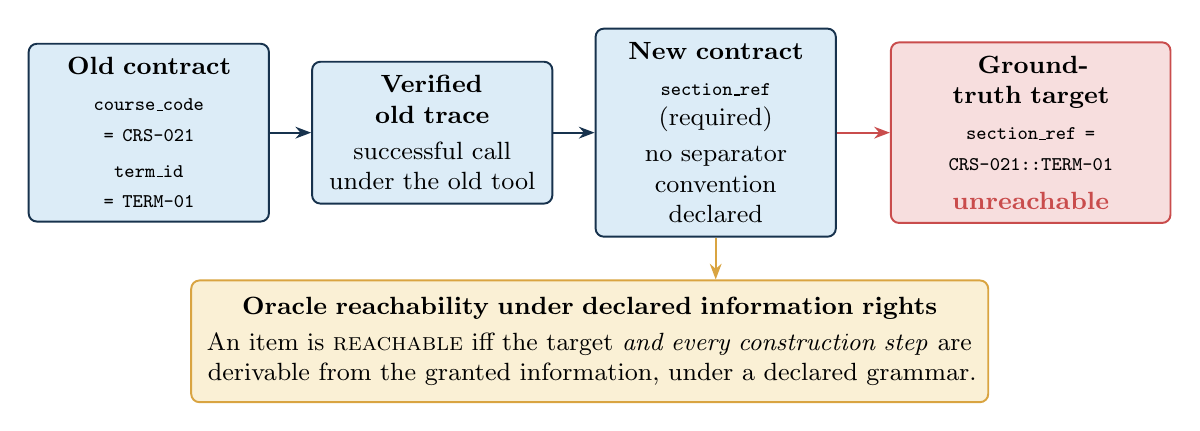
\begin{tikzpicture}[
  font=\small,
  box/.style={draw=navy,line width=0.7pt,rounded corners=3pt,
              align=center,inner sep=5pt,minimum height=15mm,text width=27mm},
  vis/.style={box,fill=paleblue},
  bad/.style={box,fill=palered,draw=unreachred,text width=32mm},
  ar/.style={-{Stealth[length=2mm]},navy,line width=0.7pt}
]
\node[vis] (old)  at (0,0)    {\textbf{Old contract}\\[2pt]
                               \texttt{\scriptsize course\_code}\\
                               \texttt{\scriptsize = CRS-021}\\[2pt]
                               \texttt{\scriptsize term\_id}\\
                               \texttt{\scriptsize = TERM-01}};
\node[vis] (tr)   at (3.6,0)  {\textbf{Verified old trace}\\[2pt]
                               successful call\\ under the old tool};
\node[vis] (new)  at (7.2,0)  {\textbf{New contract}\\[2pt]
                               \texttt{\scriptsize section\_ref}\\ (required)\\[2pt]
                               no separator\\ convention declared};
\node[bad] (tgt)  at (11.2,0) {\textbf{Ground-truth target}\\[2pt]
                               \texttt{\scriptsize section\_ref =}\\
                               \texttt{\scriptsize CRS-021::TERM-01}\\[3pt]
                               \textcolor{unreachred}{\textbf{unreachable}}};
\draw[ar] (old) -- (tr);
\draw[ar] (tr)  -- (new);
\draw[ar,unreachred] (new) -- (tgt);

\node[draw=gold,fill=palegold,line width=0.7pt,rounded corners=3pt,
      text width=0.80\linewidth,align=center,inner sep=6pt]
  (crit) at (5.6,-2.65)
  {\textbf{Oracle reachability under declared information rights}\\[2pt]
   An item is \st{reachable} iff the target \emph{and every construction step}
   are derivable from the granted information, under a declared grammar.};
\draw[ar,gold] (new.south) -- (new.south |- crit.north);
\end{tikzpicture}
\caption{The measurement problem. Each source value is visible to the method,
and the target is well formed inside the evaluator, yet the \texttt{::} join
required to build it is declared nowhere in the method's information rights.
The item is syntactically valid and epistemically empty. Values are taken from
case \texttt{G07-G-0127} of the audited register.}
\label{fig:problem}
\end{figure}

% =====================================================================
\section{Related Work}
\label{sec:related}

We position this work against five literatures. In each case the relevant
question is what information the evaluated system is allowed to use, because
that is what determines whether a ground-truth target is answerable. The first
of the five is the one this paper sits closest to, and it is where the
contribution has to be stated most narrowly.

\subsection{Benchmark-validity auditing}
\label{sec:validity}

Auditing benchmarks rather than models is an established line of work, and the
honest summary of our position is that it narrows what we can claim. Zhu
et al.\ synthesise an Agentic Benchmark Checklist from benchmark-building
experience and reported issues, and show that task-setup and reward-design
defects can distort performance estimates by up to 100\% in relative terms,
with SWE-bench Verified's insufficient tests and $\tau$-bench's acceptance of
empty responses as their worked examples~\cite{zhu2025abc}. Wang et al.\ run an
agentic auditor over 168 benchmarks in nine domains and find over 25.7\%
carrying critical issues --- ambiguous design, execution conflicts, and
incorrect ground truths --- with filtering shifting model rankings and raising
average performance on SWE-bench Verified and Terminal-Bench~2 by 9.9\% and
9.6\%~\cite{wang2026autoaudit}. Mohl et al.\ build automated transcript
scanners for four validity issues and report verified defects in five widely
used benchmarks~\cite{mohl2026transcript}. Wang et al.\ approach the same
object adversarially, presenting an eight-pattern taxonomy of benchmark
vulnerabilities and uncovering 219 distinct flaws across ten
benchmarks~\cite{wang2026benchjack}.

Closest of all is Bhat et al., who audit the validity and reproducibility of
four tool-calling benchmark families --- BFCL~v4, $\tau^2$-Bench, LiveMCPBench,
and MCP-Atlas --- and report 92 evaluator-human disagreements across 496
expert-reviewed tasks, an 18.5\% misalignment rate, alongside incorrect ground
truths, brittle state matching, and a 57.9--76.8\% spread across 23 repeated
evaluations of one LiveMCPBench setup~\cite{bhat2026benchmarking}. That work
shares our object (tool-calling benchmarks), our concern (the evaluator rather
than the agent), and our venue. Concurrently, Zhang et al.\ formalise a
\emph{double measurement confound} in which execution-critical decisions sit in
a fixed scaffold while the scorer applies criteria that need not reflect task
correctness~\cite{zhang2026doubleconfound}.

The distinction we can defend is one of position in the evaluation pipeline,
not of novelty in auditing benchmarks. Each of these audits inspects evidence
that exists only after a trajectory has been produced: transcripts, evaluator
decisions, repeated-run variance, scaffold behaviour, expert re-judgement of
completed tasks. Their question is whether the score assigned to an execution
was the right score. Ours is prior to execution and does not need a trajectory
at all: given only the information the benchmark grants before the first call,
is the expected target determined? An item can pass every post-execution check
in this literature --- a faithful evaluator, a correct reward basis, stable
reruns --- and still be unanswerable, because the defect is in what the item
withholds rather than in how the result is graded.

Mohl et al.\ make the contrast exact in one of their four criteria. They scan
for \emph{ground-truth access}: cases where an agent can reach information it
was not meant to have, inflating scores~\cite{mohl2026transcript}. The defect
we measure is the mirror image on the same axis. There, too much of the oracle
is reachable; here, not enough of it is. Both are failures of the information
boundary between the item and the method, and an audit suite that checks only
the leakage direction will pass every item in the \dfam{argument\_merge}
family of Section~\ref{sec:units}.

Two consequences follow for how this paper should be read. First, we make no
priority claim over benchmark-validity auditing, and no claim to be the first
to find incorrect ground truths in an agent benchmark --- Wang et al.\ and Bhat
et al.\ both report that class. Second, what we offer within that established
programme is specific: a pre-execution criterion, a declared information-rights
object and derivation grammar as committed artifacts, and a deterministic
per-item decision rather than expert review or an LLM judge. The cost of that
specificity is equally definite, and Section~\ref{sec:limits} states it: the
criterion decides derivability under a declared grammar, over one self-authored
benchmark.

\subsection{Agents that adapt to evolving tools}

ToolEVO enables ``active exploration and interaction of LLMs within dynamic
environments'' using Monte Carlo tree search, and supports ``autonomous
self-reflection and self-updating of tool usage based on environmental
feedback''; it introduces ToolQA-D to evaluate the impact of tool
variability~\cite{chen2025toolevo}. ContDa targets the same problem from the
documentation side, combining relation-guided exploration, which ``leverages
functionally related existing tools as anchors to probe and identify new tool
capabilities,'' with relation-aware adjustment that encodes usage preferences
and fallback options among overlapping tools~\cite{wu2026contda}.

Both systems are permitted to probe. That permission matters for our
criterion in a way that is easy to misread. We are not claiming these methods
would fail on an unreachable item; a probing agent may well observe a
\texttt{::} in a response and recover. We are claiming the opposite direction:
because those rights differ, a value recoverable by interaction does not
license a benchmark to demand the same value from a method scored before any
interaction. Reachability is a property of an item \emph{relative to a
declared rights set}, not an absolute property of the item.

\subsection{Drift benchmarks and schema-hiding architectures}

Assidiqi et al.\ benchmark reference-free LLM agent robustness under schema,
policy, and toolset drift~\cite{assidiqi2026referencefree}. This is the
closest adjacent design to ours in framing, and we position against it at the
level its title and indexed metadata support; we were unable to retrieve its
full text for verification in preparing this version, and we therefore make
no claim about its internal construction. Appendix~\ref{app:refs} records
that verification limit explicitly rather than leaving it implicit.

Tool Primitives take a different route, wrapping each tool ``with an LLM
interface that handles schema resolution and execution
internally''~\cite{jin2026toolprimitives}, so the planner never sees the raw
schema. This is a reasonable systems choice and it is orthogonal to oracle
validity rather than a solution to it. The wrapper still owns a schema, a
resolver, and execution feedback; hiding the schema from the planner
relocates the information-rights boundary instead of removing it. Under our
criterion the question simply moves: if a benchmark scores a hidden
construction convention, either the wrapper is granted what it needs to derive
that convention, or the item is unreachable for the wrapper too.

\subsection{MCP evaluation}

MCPEvol-Bench evaluates LLM agents under dynamic toolset evolution across 123
MCP servers with 11 mutation operators, reporting performance drops of 13.7\%
for GPT-5.4 and 14.4\% for Claude-Sonnet-4-6 on evolved tool
interfaces~\cite{liu2026mcpevol}. It precedes this manuscript, and we make no
claim to a first benchmark in this area. DynamicMCPBench distils successful
trajectories into path-agnostic effect checkpoints and ``scores an agent on
whether it reproduces those effects, never on the final
answer''~\cite{kaminski2026dynamicmcpbench}.

DynamicMCPBench is worth a second look, because its design partially
anticipates our concern by a different route. Scoring effects rather than a
fixed path removes one way an oracle can over-specify: the agent is no longer
penalised for reaching the right state by an unexpected sequence. Our
criterion addresses a failure that survives that fix. An effect checkpoint can
itself require a value the agent was never shown, and a path-agnostic scorer
will reject every path to it. The two mechanisms are complementary: effect
scoring loosens the path, reachability auditing validates the target.

We attempted to audit both releases directly and could not
(Section~\ref{sec:pathA}). That attempt did establish one thing we would
otherwise be asserting from an abstract: reading the MCPEvol-Bench runner at a
pinned commit shows its agent is given current tool names, descriptions, and
input schemas, receives the stringified result or error of each call truncated
to 500 characters, and continues over bounded rounds. Its rights therefore
include execution feedback and retries; ours end at the first call. Neither
setting is more correct --- they answer different questions --- but a target
that is recoverable by probing in their regime is not thereby derivable in
ours, and an auditor built for one should not be pointed at the other. This is
the concrete case behind the general point made in Section~\ref{sec:related}
about probing methods.

\subsection{API migration in software engineering}

Dig and Johnson studied API changes across four frameworks and one library and
found that breaking changes ``are not random, but tend to fall into particular
categories,'' with over 80\% of them being
refactorings~\cite{dig2006api}. More recent work applies LLMs to the same
problem: Almeida et al.\ migrate a client application to a newer SQLAlchemy
version using zero-shot, one-shot, and chain-of-thought prompting, finding
one-shot strongest~\cite{almeida2024librarymigration}; BigBag generates
executable AST transformation rules for breaking dependency updates and
transfers them across client projects, reporting a 94.3\% compilable
transformation rate and a 78.6\% single-project fix rate on 157 compilation
failures from the BUMP benchmark, dropping to 33.3\% across
projects~\cite{reyes2026bigbag}.

The distance from our setting is structural, not terminological. Those systems
transform source code and are scored by compilation or test outcomes; they may
consult repository history, compiler diagnostics, or a supplied transformation.
An agent evaluated before its first call on a live interface has none of
those. The cross-project drop BigBag reports --- 78.6\% within a project
against 33.3\% across projects --- is in fact a useful reminder for our
setting: transformation knowledge does not transfer freely even when the
transformation is explicit and the code is available. A benchmark that expects
an agent to infer an undeclared convention with far less information should
expect to be measuring something other than capability.

% =====================================================================
\section{Problem Formulation}

\subsection{Units of measurement}
\label{sec:units}

Three denominators appear throughout, and conflating them is the most common
way to misread this kind of audit. We fix them here and use them consistently.

\begin{description}[style=nextline,leftmargin=1.2em]
  \item[Graded case] One migration task, scored end to end. The audited
  benchmark has 15 graded cases in each of 12 families.
  \item[Argument-pair item] One (old argument $\rightarrow$ new argument)
  correspondence asserted by the ground truth. There are 310 of these across
  11 families; \dfam{no\_equivalent} contributes none, because it has no
  argument-pair surface.
  \item[Required-field item] One required field of a new contract that has no
  old counterpart and must be supplied from context or a literal. There are 45
  of these, across 3 families.
\end{description}

A case fails if any of its items fails, so case-level retention is bounded
above by, and generally much lower than, item-level retention. Reporting
these on a single axis would be the error this paper is about.

\subsection{Information rights}

Let $R$ denote the information rights granted to an evaluated method: the set
of artifacts and fields it may read before producing its first new-version
call. For the audited benchmark, $R$ is declared machine-readably and
contains exactly four artifacts.

\begin{center}
\small
\begin{tabular}{@{}p{0.22\linewidth}p{0.70\linewidth}@{}}
\toprule
\textbf{Granted artifact} & \textbf{Fields exposed} \\
\midrule
old contracts & tool name; description; input schema; declared input fields;
field types and descriptions; declared preconditions and effects \\
verified old traces & visible old tool calls; visible old argument names and
values; visible outputs and effects included in the trace \\
new contracts & candidate tool names; descriptions; input schemas; declared
input fields; field types and descriptions; declared preconditions and
effects \\
task context & task prose; old tool identity supplied in the task; candidate
inventory supplied in the task \\
\bottomrule
\end{tabular}
\end{center}

\medskip
Eight artifact classes are excluded by the same declaration: evaluator-only
ground truth; sandbox source and internal operations code; migration map;
new-version reference trajectory; post-call execution feedback; candidate-order
oracle; scoring code; and hidden repair annotations. The declaration is
committed at \artifact{research/gate19/information_rights.json}.

Table~\ref{tab:rights} compares this rights set against the two references an
audit needs: a method that may probe, and an oracle that sees everything. We
restrict the table to rows we can state from primary sources --- our own
committed declaration, and a published abstract --- rather than inferring the
rights of systems whose full text we did not verify.

\begin{table}[t]
\centering
\small
\caption{Information rights as an audit object. The \emph{oracle} row is an
audit reference with access to the correspondence; it is not an agent
condition and no method is evaluated under it. Rows are restricted to
settings whose rights we can state from a primary source.}
\label{tab:rights}
\begin{tabular}{@{}lccccc@{}}
\toprule
Setting & Old & Old & New & Migration & Probe before \\
        & schema & trace & schema & map & first call \\
\midrule
Audited setting (ours) & yes & yes & yes & no & no \\
Probing agent (e.g.~\cite{chen2025toolevo}) & stale & --- & via interaction & no & yes \\
Oracle (audit reference) & yes & yes & yes & yes & no \\
\bottomrule
\end{tabular}
\end{table}

\subsection{The criterion}

For a ground-truth item $g$, a declared rights set $R$, and a declared
derivation grammar $G_R$,
\[
  \operatorname{Reachable}(g \mid R, G_R)=
  \begin{cases}
    1, & \text{if the target \emph{and every construction step}}\\
       & \text{are derivable from } R \text{ under } G_R,\\[2pt]
    0, & \text{otherwise.}
  \end{cases}
\]

Three boundaries keep this criterion honest.

It is strictly \emph{weaker} than semantic correctness. A derivable target can
still be the wrong replacement, and this audit will pass it. Reachability is a
necessary condition for an item to be a valid capability test, never a
sufficient one.

It is \emph{relative to the rights set}. An item unreachable under one rights
set may be reachable under another, which is why the declaration is a committed
artifact rather than a description in prose. Changing $R$ changes the audit
result, and it should.

It is also \emph{relative to the derivation grammar}, and this is the boundary
we stated too loosely in earlier versions. The auditor is not a general
theorem prover and cannot decide arbitrary computability. It recognises the
finite rule set below and nothing else. Lower-casing, JSON re-serialisation,
arithmetic transforms, hashing, template concatenation, and unit normalisation
are all constructions a real migration might require, and $G_R$ as declared
here decides none of them: an item needing one would be classified unreachable
by the fail-closed rule. That makes the criterion conservative in a specific
direction --- it can call an item unreachable that a richer grammar would
derive --- and any reported rate is a statement about $(R, G_R)$ jointly, not
about derivability in general. Both objects are committed:
$R$ at \artifact{research/gate19/information_rights.json} and $G_R$ at
\artifact{research/gate19/derivation_grammar.json}.

\subsubsection*{The declared grammar}

Four rules admit an item, one rejects it on a named construction, and a
fail-closed rule rejects everything else. The counts are how often each fires
over the frozen 310-item register.

\begin{description}[style=nextline,leftmargin=1.2em]
  \item[identity (225)] A target equal to a visible source value is derivable.
  \item[visible\_literal (35)] A string target occurring verbatim in the
  method-visible surface is derivable.
  \item[visible\_split (0)] A target that is an explicit prefix or suffix of a
  visible source value, split by a delimiter \emph{present in that source
  value}, is derivable from the observed value. The delimiter alphabet is
  fixed and finite.
  \item[declared\_external\_derivation (0 here; 15 externally)] For externally
  sourced pairs, a hand-verified annotation may mark a derivation observable
  only when its inputs and construction rule are present in the declared source
  surface. This rule records an adjudicator's judgement, not a mechanical
  check, and Section~\ref{sec:external} reports the external sample twice
  because of it.
  \item[unobservable\_join (40)] A target formed by concatenating two distinct
  visible source values with a separator that occurs nowhere in the visible
  surface is \emph{not} derivable. This is the rule that produces every
  \st{unreachable-convention-unobservable} classification in this audit.
\end{description}

\subsubsection*{A declaration defect, and why it did not move the result}
\label{sec:ablation}

The frozen rights declaration lists three of these rules. It does not list
\texttt{visible\_literal} or \texttt{unobservable\_join}, both of which the
committed auditor evaluates. We record that as a defect in the declaration
rather than a defect in the audit, and we did not repair it by editing the
frozen artifact, since that artifact is what the frozen run was produced
under. The complete grammar is declared in a new committed file and the audit
output is bit-identical before and after it was added.

The reason the defect did not move a number is structural, and it is
checkable. \texttt{visible\_literal} is strictly weaker than
\texttt{visible\_split}: a target that is a delimiter-bounded piece of a
visible source value is necessarily also a substring of the visible surface.
Because it is evaluated first, it shadows \texttt{visible\_split} --- which is
why the declared rule fires zero times and the undeclared one fires 35. On this
register the two accept exactly the same items. We verified this by ablation
rather than by argument, re-running all 310 items under four configurations of
$G_R$:\ledger{B01--B04}

\begin{center}
\small
\begin{tabular}{@{}llrrr@{}}
\toprule
& Configuration & \st{reach} & \st{absent} & \st{conv.} \\
\midrule
V1 & As committed (literal evaluated first) & 260 & 10 & 40 \\
V2 & \texttt{visible\_literal} removed & 260 & 10 & 40 \\
V3 & \texttt{visible\_split} evaluated first & 260 & 10 & 40 \\
V4 & \texttt{visible\_literal} scoped to source values only & 260 & 10 & 40 \\
\bottomrule
\end{tabular}
\end{center}

\medskip
Per-family counts are identical across all four, and V2 and V3 reassign exactly
the 35 shadowed items to \texttt{visible\_split} with no status change. The
50/310 result does not depend on the undeclared rule. The harness is committed
at \artifact{research/gate19/ablation.py}, asserts that its default
configuration reproduces the committed auditor item for item before reporting
anything, and runs as the fifth stage of the reproduction script.

The asymmetry between \texttt{visible\_split} and the \texttt{::} join is the
crux of the whole audit. Splitting \texttt{CRS-021::TERM-01} into its parts is
derivable when the method can see that string, because the delimiter is
present in the observed value. Joining \texttt{CRS-021} and \texttt{TERM-01}
into it is not, because the delimiter is present nowhere the method may look.
This is also why \dfam{argument\_split} is clean at 40/40 while
\dfam{argument\_merge} is 0/30: the two families are mirror images, and the
mirror is not symmetric with respect to information.

A fail-closed rule governs ambiguity: if a target is not a declared field, or
a required construction convention is not evidenced by the declared surface,
the item is classified unreachable rather than assigned a likely convention.
The auditor never substitutes a guessed field, delimiter, default, or format.

% =====================================================================
\section{Audit Procedure}

\subsection{Implementation}

The auditor is offline, deterministic, and committed at
\artifact{research/gate19/auditor.py} with unit tests at
\artifact{research/gate19/tests.py}. It emits exactly three statuses.

\begin{center}
\small
\begin{tabular}{@{}p{0.33\linewidth}p{0.60\linewidth}@{}}
\toprule
\textbf{Status} & \textbf{Condition} \\
\midrule
\st{reachable} & Target field is declared, and every value and construction
step follows from $R$ under a rule of $G_R$. \\
\st{unreachable-target-absent} & The ground truth names a target field that is
not a field of any new contract the method is shown. \\
\st{unreachable-convention-unobservable} & The target field exists, but a
required construction step --- a delimiter, literal, default, ordering, or
format --- is not evidenced anywhere in $R$. \\
\bottomrule
\end{tabular}
\end{center}

\medskip
The division of labour between the rights declaration and the auditor needs
stating precisely, because the natural reading of the preceding sections is
wrong in a way that would overstate what the implementation does. The auditor
is \emph{not} a policy engine that filters raw benchmark artifacts against $R$
at run time. The rights declaration is instantiated ahead of the audit by
benchmark-specific builders, which materialise the granted surface into a
normalised register: each item carries the visible source values, the visible
text, and the declared fields of the new contract that $R$ grants for that
item. The auditor then verifies derivability over that normalised surface.
Concretely, its per-item entry point accepts the rights object but reads only
its schema identifier; what constrains the classification is the materialised
surface, not a parsed policy.

This matters for how the criterion's relativity should be read. Changing $R$
changes the audit result --- but it does so by changing what the builders
materialise, not by changing the auditor's behaviour at fixed input. The
executable form of that claim is a test: withdraw a source value from an
item's granted surface and a \st{reachable} target becomes
\st{unreachable-convention-unobservable}.\footnote{%
\artifact{research/gate19/tests.py}, \texttt{test\_rights\_instantiation\_%
controls\_the\_visible\_surface}.} An auditor generic over an arbitrary rights
policy would need machinery this implementation does not have, and we do not
claim one; what is claimed is that the audited benchmark's materialised
method-facing surface does not derive 50 of its 310 targets.

For each item, then, the auditor preserves the original record; checks
target-field presence against the visible new contract; checks value
derivability against the materialised visible surface under $G_R$; then emits a
typed status and a retain-or-exclude action. It never rewrites the original
oracle. Repair is \emph{additive}: the retained set and the full exclusion
manifest are new artifacts, and no frozen score is recomputed
(Appendix~\ref{app:procedure}).

\subsection{Audited surfaces}

The audited sandbox is self-authored and deterministic, covering renames,
argument restructuring, merges and splits, semantic near-collisions, tool
replacement, and no-equivalent controls. We do not treat it as an external
dataset, and its provenance is the central limitation of this paper
(Section~\ref{sec:limits}). The object of measurement is not the sandbox's
difficulty but whether its generated oracle is well formed under the rights
declared to the method.

Cases are not hand-written. A 291-line operator library turns sandbox contract
lineages into cases under a fixed generator seed (\texttt{20260827}), emitting
15 graded and 3 held-out cases per family; the held-out split is never scored
in the results reported here. This matters for how the results should be read.
The unreachable targets are not authoring slips scattered at random: they are
the systematic output of two mutation operators, which is why the failures
cluster perfectly in \dfam{argument\_merge} and \dfam{tool\_replacement} rather
than appearing at low rates everywhere. The \texttt{::} separator that makes
those targets underivable is produced inside the sandbox's own operations code,
for example
\begin{quote}\ttfamily\footnotesize
"section\_code": f"\{course['course\_code']\}::\{\_term\_id(args)\}"
\end{quote}
and the ground truth is constructed to match that behaviour. The evaluator and
the environment agree with each other; only the method is excluded from the
convention.

Three surfaces were audited: 310 argument-pair items across 11 families; 45
required-field items across 3 families; and, as an external sample, 20
hand-verified parent/new commit pairs from the official MCP servers
repository. A fourth surface --- public MCP-evolution benchmark releases ---
was attempted and abandoned for the reasons in Section~\ref{sec:pathA}.

\subsection{Pre-registration and integrity}

The audit and its statistical decision rule were frozen before this
manuscript. Gate~19 froze the criterion, auditor, and exclusion policy;
Gate~19-C re-ran the auditor over all 12 families and froze the power rule
before any power number was computed. Both gates recorded a hash manifest of
every input file read, re-verified at closure: 134 files unchanged for
Gate~19, and a separate 146-hash inventory unchanged for Gate~19-C
(99 protocol-surface, 30 V3 raw-artifact, and 17 V4 raw-artifact hashes).
The two counts are different inventories over different file sets and must not
be combined.\ledger{C028, C045} The full test suite passed 612 tests with 2
warnings at both closures. No frozen source, corpus, manifest, chunk store,
embedding artifact, or golden set was modified for this manuscript, with one
exception that is recorded rather than absorbed: eight frozen Gate~07 and
Gate~08 protocol artifacts had their file bytes restored to the line-ending
form their own manifest records, because Git had normalised them at an earlier
commit and they no longer hashed to it. Their parsed content is unchanged and
the manifest itself was not edited; Section~\ref{sec:repro} gives the detail.
That 134-file manifest is re-verified in full only in a working tree that also
holds the raw measurement archive, which the repository does not distribute.

% =====================================================================
\section{Results}

\subsection{Unreachability is concentrated, not diffuse}

Across the synthetic argument-pair surface, 260 of 310 items are reachable and
50 are not, or 16.1\%.\ledger{C001--C005} The headline rate is the least
informative thing about that number. Table~\ref{tab:families} shows the
distribution: on this surface nine of eleven families are clean, and all 50
unreachable items come from two families. ``Clean on this surface'' is not
``clean'': Table~\ref{tab:families}'s rightmost column already shows
\dfam{added\_required\_field} retaining 0 of 15 strict cases despite a
flawless 40/40 pair record, and Section~\ref{sec:reqfield} explains why.

\begin{table}[t]
\centering
\small
\caption{Per-family audit of the synthetic drift surface. \emph{Pairs} counts
argument-pair items; \emph{cases} counts graded migration tasks
(Section~\ref{sec:units}). \st{absent} and \st{conv.} are the two unreachable
statuses. Strict complete-call retention requires every item of a case to be
retained. The total row covers the 11 families that have an argument-pair
surface; \dfam{no\_equivalent} contributes 15 further graded cases and no pair
items, giving 12 families and 180 graded cases overall.}
\label{tab:families}
\begin{tabular}{@{}lrrrrrrr@{}}
\toprule
Family & Cases & Pairs & \st{reach} & \st{absent} & \st{conv.} & Retained & Strict \\
       &       &       &            &             &            &          & cases  \\
\midrule
\dfam{added\_required\_field}         & 15 & 40 & 40 & 0  & 0  & 40 & 0/15 \\
\dfam{argument\_merge}                & 15 & 30 & \textbf{0}  & 0  & \textbf{30} & \textbf{0}  & 0/15 \\
\dfam{argument\_rename}               & 15 & 20 & 20 & 0  & 0  & 20 & 15/15 \\
\dfam{argument\_split}                & 15 & 40 & 40 & 0  & 0  & 40 & 15/15 \\
\dfam{multiple\_old\_to\_one\_new}    & 15 & 30 & 30 & 0  & 0  & 30 & 15/15 \\
\dfam{multiple\_simultaneous\_renames}& 15 & 40 & 40 & 0  & 0  & 40 & 15/15 \\
\dfam{no\_equivalent}                 & 15 & --- & --- & --- & --- & --- & --- \\
\dfam{one\_old\_to\_multiple\_new}    & 15 & 30 & 30 & 0  & 0  & 30 & 15/15 \\
\dfam{output\_restructure}            & 15 & 15 & 15 & 0  & 0  & 15 & 15/15 \\
\dfam{semantic\_near\_collision}      & 15 & 15 & 15 & 0  & 0  & 15 & 15/15 \\
\dfam{tool\_rename}                   & 15 & 15 & 15 & 0  & 0  & 15 & 15/15 \\
\dfam{tool\_replacement}              & 15 & 35 & \textbf{15} & \textbf{10} & \textbf{10} & \textbf{15} & 0/15 \\
\midrule
\textbf{Total (11 pair families)}    & 165 & \textbf{310} & \textbf{260} & \textbf{10} & \textbf{40} & \textbf{260} & --- \\
\bottomrule
\end{tabular}
\ledger{C001--C018}
\end{table}

Figure~\ref{fig:reachability} shows the same distribution visually alongside
the real-version sample.

% ---------------------------------------------------------------- fig 2
\begin{figure}[t]
\centering
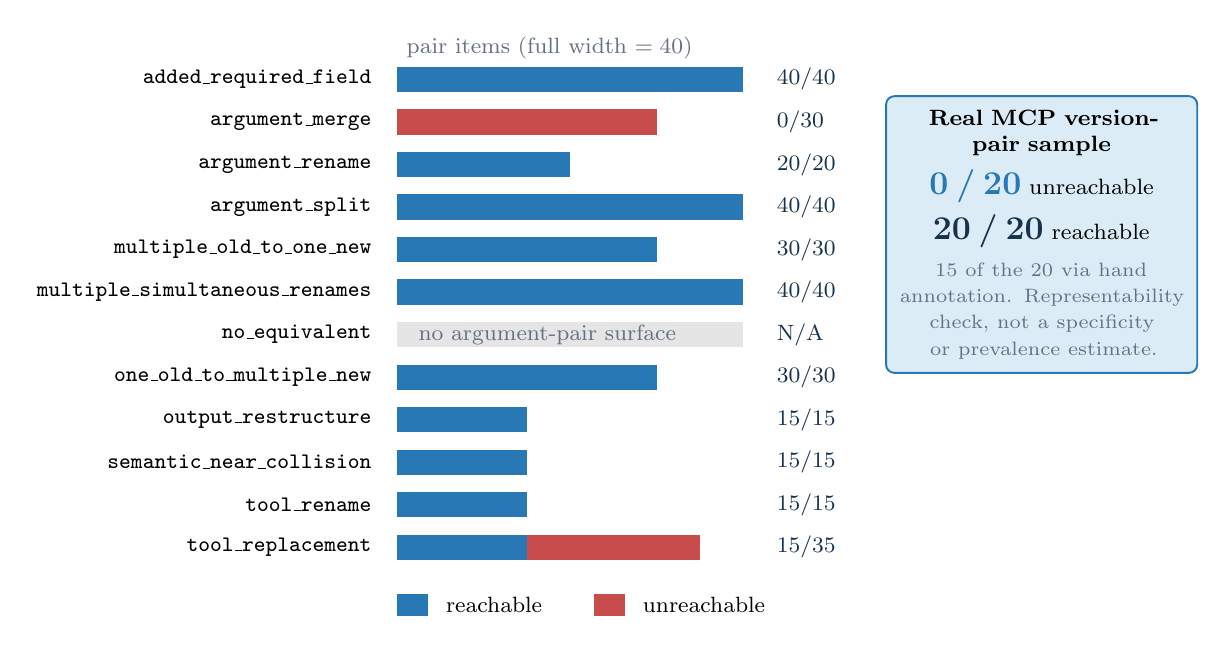
\begin{tikzpicture}[font=\footnotesize,x=1mm,y=1mm]
\def\rowh{5.4}
% axis note
\node[anchor=west,slate] at (48,4) {pair items (full width $=40$)};
\foreach \i/\name/\r/\u/\lab in {
  0/{\texttt{added\_required\_field}}/40/0/{40/40},
  1/{\texttt{argument\_merge}}/0/30/{0/30},
  2/{\texttt{argument\_rename}}/20/0/{20/20},
  3/{\texttt{argument\_split}}/40/0/{40/40},
  4/{\texttt{multiple\_old\_to\_one\_new}}/30/0/{30/30},
  5/{\texttt{multiple\_simultaneous\_renames}}/40/0/{40/40},
  7/{\texttt{one\_old\_to\_multiple\_new}}/30/0/{30/30},
  8/{\texttt{output\_restructure}}/15/0/{15/15},
  9/{\texttt{semantic\_near\_collision}}/15/0/{15/15},
  10/{\texttt{tool\_rename}}/15/0/{15/15},
  11/{\texttt{tool\_replacement}}/15/20/{15/35}}
{
  \node[anchor=east] at (46,-\i*\rowh) {\name};
  \pgfmathsetmacro{\rw}{\r*1.1}
  \pgfmathsetmacro{\uw}{\u*1.1}
  \ifdim\rw pt>0pt
    \fill[reachblue] (48,-\i*\rowh-1.6) rectangle (48+\rw,-\i*\rowh+1.6);
  \fi
  \ifdim\uw pt>0pt
    \fill[unreachred] (48+\rw,-\i*\rowh-1.6) rectangle (48+\rw+\uw,-\i*\rowh+1.6);
  \fi
  \node[anchor=west,navy] at (95,-\i*\rowh) {\lab};
}
% no_equivalent row
\node[anchor=east] at (46,-6*\rowh) {\texttt{no\_equivalent}};
\fill[black!10] (48,-6*\rowh-1.6) rectangle (92,-6*\rowh+1.6);
\node[anchor=west,slate] at (49.5,-6*\rowh) {no argument-pair surface};
\node[anchor=west,navy] at (95,-6*\rowh) {N/A};

% legend
\fill[reachblue] (48,-12.4*\rowh-1.2) rectangle (52,-12.4*\rowh+1.6);
\node[anchor=west] at (53,-12.4*\rowh+0.2) {reachable};
\fill[unreachred] (73,-12.4*\rowh-1.2) rectangle (77,-12.4*\rowh+1.6);
\node[anchor=west] at (78,-12.4*\rowh+0.2) {unreachable};

% control panel
\node[draw=reachblue,fill=paleblue,line width=0.7pt,rounded corners=3pt,
      align=center,inner sep=5pt,text width=36mm,anchor=north west]
  at (110,-2) {\textbf{Real MCP version-pair sample}\\[4pt]
  {\large\textbf{\textcolor{reachblue}{0 / 20}}} unreachable\\[3pt]
  {\large\textbf{\textcolor{navy}{20 / 20}}} reachable\\[4pt]
  \textcolor{slate}{\scriptsize 15 of the 20 via hand annotation.
  Representability check, not a specificity or prevalence estimate.}};
\end{tikzpicture}
\caption{Oracle reachability across the synthetic drift families. Blue is
derivable pair items, red is unreachable pair items. All 50 unreachable items
fall in \dfam{argument\_merge} and \dfam{tool\_replacement}. The
\dfam{no\_equivalent} family has no argument-pair denominator and is not
assigned an artificial one. The real-version sample is shown separately
because it is a different population, not a comparison arm, and its panel
records how many of its 20 acceptances rest on hand adjudication rather than
on a mechanical rule (Section~\ref{sec:external}).}
\label{fig:reachability}
\end{figure}

The two failing families fail for different reasons, and the distinction is
diagnostic rather than cosmetic. \dfam{argument\_merge} fails entirely on
construction: all 30 items name a field that exists, and all 30 require the
undeclared \texttt{::} join. \dfam{tool\_replacement} fails in both available
ways --- 10 items name a field that is absent from the new contract
altogether, and 10 more require the same undeclared join. An author reading
only an aggregate unreachability rate would learn that something is wrong;
reading the typed statuses tells them that one generator mutation invents
fields and another invents conventions, which are separate bugs with separate
fixes. Appendix~\ref{app:register} lists all 35 items of that family so the
15/10/10 split can be checked by hand rather than taken on trust.

\subsection{Required fields are a second, independent defect surface}
\label{sec:reqfield}

The argument-pair audit is not the whole oracle. New contracts also declare
required fields with no old counterpart, and these were audited separately:
25 of 45 items are reachable and 20 are not. All 15 \dfam{added\_required\_field}
items require boolean acknowledgement values (\texttt{consent\_ack},
\texttt{honor\_code}, \texttt{payment\_ack}) that appear as neither explicit
literals nor declared defaults; 5 of 25 \dfam{tool\_replacement} items require
the literal \texttt{approved} without that value appearing in the visible
contract. The 5 \dfam{argument\_split} required fields are derivable by
identity.

The consequence is severe and is the reason the two surfaces must be reported
together. Complete-call scoring requires every field of a call to be correct,
so a single unreachable required field invalidates the whole case even when
every argument pair in it is clean. Strict complete-call retention is
therefore 0/15 for \dfam{added\_required\_field} --- a family whose pair
surface is perfectly clean at 40/40 --- and 0/15 for
\dfam{tool\_replacement}.\ledger{C018} The retained 15 pair items in
\dfam{tool\_replacement} must accordingly never be presented as a repaired
end-to-end performance surface. They support reachability and power analysis
only.

\subsection{An external sample, reported with its adjudication exposed}
\label{sec:external}

A criterion that marked every version change as defective would be useless, and
we assembled an external sample to check that. Twenty parent/new commit pairs
were taken from the official MCP servers repository, chosen and checked by
hand, with all 20 commit objects and all 20 changed artifact paths verified
against a local clone. All 20 are representable as audit items, and the auditor
returns 20 \st{reachable} and 0 unreachable.\ledger{C019}

Earlier versions of this manuscript called that a negative control and
concluded from it that the auditor does not flag ordinary interface evolution.
That conclusion does not survive inspection of what produced the 20, and we
withdraw it. Under the declared grammar, 15 of the pairs are admitted by
\texttt{declared\_external\_derivation} --- the rule that accepts a
hand-supplied annotation marking the derivation observable --- and only 5 by
\texttt{visible\_literal}, a mechanical rule.\ledger{B05} The annotation comes
from the same adjudication pass that assigned each pair its hand judgement, so
for three quarters of the sample the auditor is reporting the adjudicator's
conclusion back. Running the sample with the annotation withheld makes the
dependence explicit: 5 \st{reachable} and 15
\st{unreachable-convention-unobservable}.\ledger{B06}

The remaining 5 are worth naming rather than banking, because they are weaker
than the count suggests. In three of them the target value \emph{is} the new
tool's own registered name, which necessarily appears in the diff that registers
it. A fourth target is the schema status word \texttt{required}, and the fifth a
resource description string. These are true mechanical derivations under the
declared grammar, and three of them are close to tautologies. We report them as
the floor of what this sample establishes, not as five independent successes.

What the sample does show is that real, externally sourced interface changes
can be normalised into the audit schema at all --- which the failed adaptation
of Section~\ref{sec:pathA} shows is not automatic --- and that nothing in this
sample reproduced the local defect. What it does not show is auditor
specificity, because a specificity estimate needs items whose reachability was
decided without the adjudicator's help, and 15 of these were not. It also does
not estimate how often unreachable oracles occur in real API evolution, and it
does not establish that synthetic generation is the only source of such
defects. The sample is purposive, drawn from a single repository, and small.
The strengthening this most needs is not thirty pairs instead of twenty; it is
a subset whose targets are decidable under \texttt{identity},
\texttt{visible\_literal}, or \texttt{visible\_split} alone, with no
\texttt{declared\_external\_derivation} anywhere in it. We did not build that
subset for this version and do not claim its result in advance.

\subsection{A published evolution register that an oracle auditor still cannot
consume}
\label{sec:pathA}

We tried to run the same audit on a public MCP-evolution benchmark. The attempt
failed, and the shape of the failure is more informative than the attempt would
have been had it succeeded.

Our first pass looked at the MCPEvol-Bench task file, found questions,
trajectories, tool calls, and evaluation results, and concluded that no
old/new correspondence register was published. That conclusion was wrong, and
we had reached it by opening the wrong file. The repository does publish one:
four cumulative mutation-stage files totalling 2,124,315 bytes, pinned here at
commit \sha{888c779a0fe735f612ca62bdd1fdd7c9e6bf8701}. They contain 347 mutated
server entries across 89 distinct servers, typed by mutation: 152
\texttt{DESC}, 141 \texttt{PARAM}, and 54 \texttt{TOOL}.

It is still not auditable by our criterion, and the reasons are specific.
\texttt{PARAM} entries name the parameters added and supply 357 source-code
diff hunks, but no normalized old and new argument sets and no expected call
carrying a target value; recovering a schema from them would mean inferring it
from implementation code, which is weaker evidence than a declared contract and
which we declined to do. \texttt{DESC} entries pair descriptions, which is not
an argument-target surface at all. \texttt{TOOL} entries carry prose summaries,
lists of knock-on adjustments, and 22 complete new tool configurations, none
with an old/new correspondence. A \texttt{task\_idx} field sits on server
entries with 73 distinct values in the range 0--84, but we could not verify a
join from it to the task file's own index, and we did not treat an unverified
join as one. Every record was refused by the adapter; none became an auditable
item. That is a feasibility result, and it yields \emph{no} external
reachability rate --- zero converted items is not zero unreachable items, and
the two must not be confused.

Two observations from the survey are worth more than the failed audit.

First, the \texttt{parameter\_additions} surface across those 141
\texttt{PARAM} entries contains 312 parameter items, of which \textbf{0 are
required} and 312 are optional. Two further required additions appear on a
separate \texttt{parameter\_changes} surface, and two required fields appear
among 11 removals. Within the surface that most closely corresponds to our own
\dfam{added\_required\_field} family --- the family whose 15 hidden required
acknowledgement values drive its strict retention to 0/15 --- this benchmark
adds no required parameter at all. Its parameter mutations are
backward-compatible by construction.

Second, and more fundamentally, their agent does not operate under our rights.
Reading their runner at the same pinned commit: the agent receives current tool
names, descriptions, and input schemas plus task context; after each call the
runner appends the stringified result or error, truncated to the first 500
characters, to the next request; and the episode continues to a bounded number
of rounds. That is an interactive, current-schema setting. Ours is a
pre-execution, old/new setting scored on the first call. Section~\ref{sec:units}'s
point that reachability is relative to a declared rights set is not a
hypothetical distinction between our work and theirs --- it is the reason the
same auditor cannot be pointed at their register and is not entitled to try.

The recommendation we drew from the earlier, mistaken reading was that
benchmarks should publish their correspondence register. MCPEvol-Bench does.
The corrected and narrower recommendation is that publishing change records is
not sufficient for external oracle checking: \emph{an oracle becomes externally
checkable when the correspondence is normalized into old and new argument sets
and carries the expected target value}, which is a stronger requirement than
publishing a changelog and a harder one to meet.

\subsection{A claim in our own risk register was wrong}
\label{sec:risk0022}

The audit began because five graded \dfam{tool\_replacement} cases require the
\texttt{::} join. Our project risk register had recorded a mechanism for what
happened next: that the frozen baselines which scored well in that family had
guessed the unstated convention. We checked the raw rows and that claim does
not survive.

Extraction over the frozen prediction rows for the five affected cases
(\texttt{G07-G-0127}, \texttt{G07-G-0130},
\texttt{G07-G-0133}, \texttt{G07-G-0136}, and
\texttt{G07-G-0139}) across 17 baseline arms yields 85
effective rows. Of those, 0 contain a literal \texttt{::}, 3 use a different
separator, and 82 contain no join at all.\ledger{C020, C021} The three
non-empty constructions are \texttt{"CRS-007-TERM-02"} and a two-order
hyphen-join from \texttt{llm\_old\_new\_history} on \texttt{openai/gpt-oss-20b},
and the template string \texttt{"\$\{course\_code\}-\$\{term\_id\}"} from
\texttt{llm\_reasoning} on the same model. In the frozen first-attempt score
matrix, no arm scores a success on any of the five cases; the matrix contains
only zeros and structurally non-applicable cells.\ledger{C022}

The real explanation is a distinction between two scorers that we had not
separated. The argument-mapping scorer compares argument-name quadruples:
\begin{quote}\ttfamily\footnotesize
correct\_args = expected\_args \& predicted\_args
\end{quote}
so it can award mapping credit for correctly \emph{naming} \texttt{section\_ref}
without any value being constructed. First-attempt execution scoring is
stricter, comparing the produced argument dictionary against the exact
expected input and returning \texttt{wrong\_arguments} otherwise. Family-level
successes were therefore real, but they occurred on other cases in the family;
the register had attributed them to the hidden cases without checking the raw
rows.

We report this for two reasons. It is a correction we owe our own record. It
is also the clearest illustration of the paper's thesis that we have: a
plausible mechanism story survived in a risk register for weeks because
nobody re-read the rows, and the story was about capability where the evidence
was about scorer granularity.

\subsection{A diagnostic probe, reported with its ambiguity intact}
\label{sec:probe}

A separately authorised probe asked whether a model emits \texttt{::} when a
join is required but the separator is withheld. The chance baseline was frozen
before measurement as uniform over nine plausible separators
(\texttt{::}, \texttt{:}, \texttt{|}, \texttt{/}, \texttt{-}, \texttt{\_},
\texttt{.}, \texttt{\~{}}, \texttt{,}), giving
$P(\texttt{::}) = 1/9 = 0.1111$.\ledger{C023} The probe dispatched exactly 60
requests to \texttt{nvidia/nemotron-3-super-120b-a12b:free} with no fallback
model, a free-catalogue guard, a 3.2\,s minimum request interval, and
reasoning effort disabled. It obtained 57 valid JSON outputs and 3 provider
failures.\ledger{C024, C025}

\begin{center}
\small
\begin{tabular}{@{}lrrrr@{}}
\toprule
Stratum & Dispatched & Valid JSON & \texttt{::} rate & Exact-gold rate \\
\midrule
Hidden sandbox \texttt{::} convention & 30 & 28 & 0.0000 & 0.0000 \\
Hidden arbitrary separator            & 30 & 29 & 0.0000 & 0.1379 \\
\bottomrule
\end{tabular}
\end{center}

\medskip
Both \texttt{::} rates are zero.\ledger{C026, C027} We report the second
column rather than omitting it, because it complicates the tidier reading: in
the arbitrary-separator stratum the model matched the exact withheld separator
in 4 of 29 valid outputs, a rate of 0.1379 that sits close to the 0.1111
chance baseline. The honest summary is that the probe found no evidence of a
\texttt{::} prior and no evidence of anything better than chance in the
arbitrary condition, at a sample size too small to distinguish 0.1379 from
0.1111 in any case. The probe is diagnostic only. It is not a capability
measurement, and a zero result at $n=28$ is not evidence of absence.

\subsection{Repairing the oracle cost more power than it recovered}
\label{sec:power}

Gate~19-C pre-registered a two-sided two-sample normal approximation for
independent proportions with equal $n$ per arm, no continuity correction,
$\alpha = 0.05$, target power $0.80$, and a practically meaningful absolute
difference of $0.20$.\ledger{C032} The baseline anchor for each surface is the
strongest applicable direct-LLM arm against the strongest applicable
offline/control arm under the frozen scoring rule; the pooled $\bar{p}$ is
weighted by retained $n$. Table~\ref{tab:power} gives the result.

\begin{table}[t]
\centering
\small
\caption{Power consequences of the reachability repair, over retained
argument-pair items. MDE is the smallest absolute arm difference detectable at
$\alpha=0.05$ with power $0.80$ at the stated $n$. Every MDE exceeds the
pre-registered effect of $0.20$.}
\label{tab:power}
\begin{tabular}{@{}lrrrrrr@{}}
\toprule
Surface & Retained & $\bar{p}$ & MDE & Power at & Required & Wilson width \\
        & $n$/arm  &           &     & $\Delta=0.20$ & $n$/arm & at $\bar{p}$ \\
\midrule
\dfam{argument\_split}   & 40 & 0.3667 & 0.2975 & 0.4578 & 90 & 0.2862 \\
\dfam{tool\_replacement} & 15 & 0.2667 & 0.4348 & 0.2300 & 76 & 0.4105 \\
pooled retained         & 55 & 0.3394 & 0.2503 & 0.6029 & 87 & 0.2429 \\
\bottomrule
\end{tabular}
\ledger{C029--C034}
\end{table}

The observed anchors show why the intervals dominate the design. On
\dfam{argument\_split}, the direct arm (\texttt{llm\_old\_new\_history} on
\texttt{openai/gpt-oss-120b}) is 11/15 $=0.7333$ with a Wilson 95\% interval
of $[0.4805, 0.8910]$, against an offline arm (\texttt{lexical\_name},
deterministic) of 0/15 $=0.0000$ with $[0.0000, 0.2039]$. On
\dfam{tool\_replacement}, the direct arm (\texttt{llm\_reasoning} on
\texttt{openai/gpt-oss-20b}) is 8/15 $=0.5333$ with $[0.3012, 0.7519]$ against
the same 0/15 offline arm.\ledger{C035--C038}

At $n=15$, even the zero-success interval has full width 0.2039 --- already
wider than the entire pre-registered 0.20 effect band --- and the non-zero arms
are wider still, at 0.4507 and 0.4105. Reaching the meaningful effect at 80\%
power would require 90 items per arm for \dfam{argument\_split}, 76 for
\dfam{tool\_replacement}, and 87 pooled. The planned comparative campaign was
cancelled on this basis before it consumed any provider budget.

This is a design decision, not a null result. No comparison ran under the
repaired oracle, so nothing here says competing methods are equivalent; it
says the retained surface could not have resolved the effect we had committed
to detecting. The tempting escape --- manufacturing more synthetic cases to
reach $n=90$ --- is precisely the mechanism that produced the unreachable
items in the first place. Expanding the real version-pair set is the safer
direction, but 20 clean pairs do not convert to 90 scoreable items at one item
per pair, and the conversion rate has to be measured rather than assumed.

% =====================================================================
\section{Deployed Case Study}

The audit discipline described above was maintained inside an operational
system, and we include that context briefly to show the conditions under which
the artifacts were produced. The repository's deployed retrieval-augmented
generation service runs on managed cloud infrastructure; at the closure
receipt used for this manuscript, revision \texttt{vietragops-api-00021-teb}
held 100\% of traffic, and its readiness surface reported 698 chunks across 38
documents with the dense retrieval backend active.\ledger{C041, C042} The same
receipt records a release-bound build guard, authenticated health and
readiness checks, and an explicit refusal path.

Nothing in that deployment validates the synthetic oracle or supplies external
benchmark evidence, and no production call was made in support of any result
reported here. The case study is deliberately short: the service's retrieval
stack, document pipeline, and provider routing are engineering details, not
contributions of this paper.

% =====================================================================
\section{Threats to Validity and Limitations}
\label{sec:limits}

\subsection{Construct and external validity}

\textbf{The audited benchmark is self-authored.} Contribution~2 measures a
controlled local construction, not field prevalence. The concentration of all
50 failures in two mutation families points at this generator rather than at
benchmark design in general. The real-version sample found no unreachable
item, but it is small, purposive, drawn from one repository, and --- as
Section~\ref{sec:external} sets out --- adjudicated by hand for 15 of its 20
pairs, so it constrains representability rather than specificity.

\textbf{The criterion is relative to a declared grammar, and that grammar is
small.} $\operatorname{Reachable}(g \mid R, G_R)$ is not a claim about what is
computable from $R$. $G_R$ recognises identity, a visible literal, a
delimiter-bounded split over a fixed delimiter alphabet, and a hand-declared
external derivation; it decides nothing about case folding, serialisation,
arithmetic, hashing, or documented template concatenation. Under the
fail-closed rule an item requiring any of those is classified unreachable, so
the criterion errs toward calling items defective, and a richer $G_R$ could
only lower the reported rate. The 16.1\% figure should be read as a property
of this benchmark under this rights set \emph{and} this grammar. We think the
50 items reported here would survive a richer grammar --- 40 of them fail on a
separator that is absent from the visible surface by construction, and no
grammar can derive a symbol it has never seen --- but that is an argument, not
a measurement, and we have not run it.

\textbf{A declaration defect was found in the frozen rights object.} The frozen
declaration listed three derivation rules; the committed auditor evaluates
five. Section~\ref{sec:ablation} reports this, the ablation showing the
headline is invariant under four configurations of the grammar, and the
decision to declare the complete grammar in a new artifact rather than edit the
frozen one. We note the failure mode as well as the repair: the declaration and
the implementation were written to be read together and drifted apart anyway,
which is the same class of defect this paper documents in
Section~\ref{sec:risk0022}, and it was found by an external reader rather than
by us.

We are equally careful about the failed external audit of
Section~\ref{sec:pathA}. It does not show that the benchmark we examined shares
this defect, and it does not show that it avoids it: no record could be
converted into an auditable item, so no rate exists in either direction. What
it does show is that one published benchmark in this space adds no required
parameters and evaluates interactively, a design under which the
pre-execution defect class we measure does not arise. One benchmark is not the
field. A reader should take from
this paper that benchmark authors can run this audit, not that other
benchmarks share this defect.

\textbf{The criterion detects underivability only.} It says nothing about
semantic wrongness, side effects, or behavioural equivalence. A derivable
target can still be a poor replacement and this audit will pass it. Some real
migrations genuinely require probing, documentation, or human judgement; those
belong in a different information-rights condition, not forced into a
pre-execution score and then marked unreachable.

\subsection{Statistical validity}

\textbf{The power analysis mixes units.} This is the sharpest internal
limitation and we state it plainly. The power calculation runs over retained
argument-pair item counts, while first-attempt execution scoring is
case-level. The two denominators are not interchangeable
(Section~\ref{sec:units}). Because case-level retention is strictly lower than
item-level retention on the affected families --- 0/15 against 15/35 for
\dfam{tool\_replacement} --- the mismatch makes our cancellation decision more
conservative, not less: the case-level surface is smaller than the surface the
power calculation assumed. A future paired design would need its own analysis.

\textbf{The intervals are wide and the anchors are historical.} The 15-item
arms carry Wilson widths between 0.2039 and 0.4507. The anchors in
Table~\ref{tab:power} are frozen Gate~07 measurements used as inputs to a
planning calculation; they are not repaired-lane performance estimates and
must not be quoted as such. A separate recorded limitation notes that the
\dfam{argument\_split} first-attempt Wilson upper bound reaches 0.9333 against
a 0.90 saturation bar,\ledger{C039} so we claim neither stable end-to-end
saturation nor general model inability.

\textbf{The power model is an approximation used outside its comfortable
range.} The pre-registered rule uses a two-sample normal approximation for
independent proportions. At $n=15$ with an observed arm rate of exactly zero,
that approximation is not trustworthy on its own, and we do not rest the
decision on it. The decisive quantity is the interval, not the MDE: a
zero-success Wilson interval of width 0.2039 is already wider than the entire
0.20 effect band, and no choice of approximation repairs a surface that small.
Reporting the MDE table alongside it is a statement of what the frozen rule
computed, not a claim that the normal approximation is valid at these counts.

\subsection{Internal validity and disclosure}

\textbf{Design-time oracle exposure.} While scoping the earlier method gate,
the ground truth of three graded cases (\texttt{G07-G-0073},
\texttt{G07-G-0127}, \texttt{G07-G-0199}) was read before the development
discipline was tightened to held-out cases only.\ledger{C040} No case
identifier, family label, or oracle field is present in the method code and a
test enforces that, but the design was not authored in complete ignorance of
three graded cases. We disclose this rather than claim a clean room --- and we
note that \texttt{G07-G-0127} is among the exposed cases and is also the
example used in Figure~\ref{fig:problem}.

\textbf{A prior negative result is retained, not buried.} The preregistered
alignment-method result of Gate~08 was negative and remains final. The present
audit does not repair, rescore, or reverse it, and no comparative algorithmic
campaign is concealed behind this measurement paper. The subsequent campaign
was cancelled for the documented power reason in Section~\ref{sec:power} and
not after seeing an unfavourable outcome.

\textbf{Self-audit.} The auditor, the benchmark, and the risk register that
the audit corrected all originate with the same author. We have tried to
compensate through pre-registration, hash-frozen inputs, typed outputs,
item-level traceability, and a packaged reproduction path
(Section~\ref{sec:repro}) --- but every one of those is something the author
can do alone, and none of them substitutes for a second party running the
auditor.

We want to be exact about what the reproduction harness does and does not
establish, because the distinction is the same one this paper is about. Running
it confirms that the committed audit artifacts are the deterministic output of
the committed auditor over the committed inputs, and that neither has drifted.
It does not make the result independent: the script, the auditor, the
benchmark, and the expected values all come from the same source, so a shared
error would reproduce perfectly. \emph{At the time of writing, no party outside
this project has run the auditor.} A reproduction that would count is one where
someone else executes it and reports what they get, and we would rather state
that this has not happened than let an automated green result stand in for it.

\subsection{Hostile questions, answered}

\emph{Is this just test-set validity restated?} It is adjacent to that
literature and does not replace it. What is operational here is the
combination of a declared rights object, a declared derivation grammar,
per-item auditing of both field presence and construction derivability, typed
failure classes, a fail-closed rule, and a committed implementation. We claim a
checkable procedure, not a new theory of validity.

\emph{Benchmark-validity auditing already exists. What is left?} The position
in the pipeline, and nothing more (Section~\ref{sec:validity}). Existing audits
read evidence produced by an execution --- transcripts, evaluator decisions,
rerun variance --- and ask whether the score was right. This one runs before
any execution and asks whether the expected answer is determined by what the
item supplies. An item can be graded perfectly and still be unanswerable.

\emph{The auditor evaluated a rule your rights file did not declare. Why should
the 50 stand?} Because the result is invariant under removing that rule,
reordering it, and restricting its scope, and because the rule it shadowed
accepts exactly the same 35 items (Section~\ref{sec:ablation}). The defect is
real and it is in the declaration; had the ablation moved a count, the honest
report would have been a different number, not a different framing.

\emph{Does the 20-pair sample support a synthetic-versus-real claim?} No, and
we do not make one. It shows the audit schema can represent real version
changes. Fifteen of its twenty acceptances rest on hand adjudication, which is
why we no longer describe it as a negative control.

\emph{Your reproduction script exits zero, but a clone can only check 47 of the
134 manifest entries. Is that a pass?} It is a partial pass, and the harness
now says so in those words rather than reporting a clean run. The 87 it cannot
check are the raw measurement archive, which is too large to distribute in the
repository; we state the split in Section~\ref{sec:repro} instead of leaving a
reader to find it. The distinction that matters is that no reachability number
depends on those 87 files: the 310-item register is rebuilt from the committed
generator, so stages 3 and 5 are byte-identical from a bare clone. We also
found, and report, that eight frozen artifacts had stopped hashing to their own
manifest --- which is the failure mode this paper is about, occurring in our
own repository.

\emph{Is the cancelled campaign a null result in disguise?} No comparison was
run, so there is no null to disguise. The power analysis says the planned
comparison could not have resolved the pre-registered effect on the retained
surface.

\emph{What makes this more than a project report?} The transferable objects
are the criterion, the offline auditor, the typed failure classes, the
declared rights object, and the item-level evidence ledger. The deployment
narrative is bounded to one short section precisely so that it cannot carry
weight it has not earned.

% =====================================================================
\section{Reproducibility and Traceability}
\label{sec:repro}

The public repository is \url{https://github.com/Dat071104/vietragops}. Four
tags pin four different things and conflating them would misrepresent what is
frozen.

\begin{center}
\small
\begin{tabular}{@{}p{0.30\linewidth}p{0.62\linewidth}@{}}
\toprule
\textbf{Tag} & \textbf{What it denotes} \\
\midrule
\texttt{gate10-paper-v1-20260911} & \textbf{Measurement evidence freeze.} The
Gate~07, 08, 19, and 19-C artifacts from which every number in
Sections~\ref{sec:units}--\ref{sec:power} derives. Not modified since; the
reproduction harness re-verifies it at every run. \\
\texttt{gate21-paper-v2-20260912} & Adds the external survey of
Section~\ref{sec:pathA} and the version~2 manuscript text. \\
\texttt{gate22-paper-v3-20260914} & Adds the declared derivation grammar, the
rule-ablation harness and its result, four auditor tests, and the version~3
text. Superseded before submission and kept rather than moved. \\
\texttt{gate22-paper-v31-20260916} & \textbf{Manuscript artifact tag for this
version.} Adds the reproduction repairs of this section --- the byte-exactness
pinning, the eight restored protocol artifacts, and the partial-manifest
reporting --- and the text describing them. No measured value changed. \\
\bottomrule
\end{tabular}
\end{center}

\medskip
The citable identifier for this version of the manuscript is
\texttt{gate22-paper-v31-20260916}. The superseded \texttt{gate22-paper-v3-\allowbreak
20260914} is left in place rather than moved, because a tag that has been
published is a record of what was claimed at that moment and rewriting it would
be the same move this paper argues against. Later commits may refine the
repository without changing what any of the four tags denotes.

Every numeric claim in this paper carries a superscript key into a committed
evidence ledger, \artifact{gates/baselines/GATE_10_EVIDENCE_LEDGER.json},
which records for each claim its value, whether it is observed or derived, the
producing gate, the source artifact path, that artifact's commit, its SHA-256,
and a locator within the artifact. Appendix~\ref{app:traceability} lists the
artifacts with full commit hashes; Appendix~\ref{app:claims} maps each claim
key to its source. Numbers appearing in this version that were not in the
frozen ledger are recorded in an addendum shipped with the manuscript source
and are marked as such in Appendix~\ref{app:claims}.

The auditor is offline and deterministic. It needs neither network access nor
provider credentials, and it is re-run from the repository root as

\begin{quote}\ttfamily\footnotesize
python -m research.gate19.auditor \\
\hspace*{2em}{-}{-}rights research/gate19/information\_rights.json \\
\hspace*{2em}{-}{-}output <path>
\end{quote}

with \texttt{{-}{-}input} omitted so that the frozen Gate~07 items are rebuilt
from the generator rather than read from a cached file.

A single-command harness, \artifact{scripts/reproduce.py}, runs the whole check
and is documented in \artifact{REPRODUCE.md}. It imports only the Python
standard library and this repository's own modules: no third-party package, no
virtual environment, no GPU, and no network. In five stages it runs the
auditor's ten unit tests, re-verifies the frozen input manifest, regenerates
the 310-item synthetic audit, regenerates the 20-pair external sample, and
re-runs the four-configuration rule ablation of
Section~\ref{sec:ablation}; it then compares each regenerated artifact against
its committed counterpart by SHA-256. On a stock CPython interpreter the run
takes roughly fifteen seconds. What that establishes, and what it does not, is
set out in Section~\ref{sec:limits}.

What a reader who clones the repository can check is not quite all of that, and
the difference is worth stating here rather than leaving it to be discovered.
Stages 1, 3, 4, and 5 reproduce in full from a clone: the ten unit tests pass,
and the regenerated synthetic audit, external sample, and rule ablation are
byte-identical to their committed counterparts. Stage 2 is partial. The
manifest has 134 entries, of which 87 are the raw Gate~07 and Gate~08
measurement archive --- roughly 107\,MB of request ledgers, per-item traces,
and router state. That archive is excluded from the Git repository and is
carried by no tag, so a clone holds the other 47 entries and not those. The
harness verifies the 47, reports the 87 as not verified together with the
reason, and records in its summary that stage 2 was partial;
\texttt{{-}{-}require-full-manifest} turns the absence into a failure for a
working tree that does hold the archive. The archive is available from the
authors on request. A reader who wants the manifest checked end to end needs
it; a reader who wants the reachability result checked does not, because the
310-item register is rebuilt from the committed generator rather than read from
the archive.

Both properties were established by cloning the repository into a fresh working
tree and running the harness there, rather than only in the tree that produced
it. That check is also what exposed a defect in the repository itself: the
committed form of eight frozen Gate~07 and Gate~08 protocol artifacts had been
normalised to Unix line endings by Git at an earlier commit, so those eight no
longer hashed to the values their own frozen manifest records. Their bytes are
restored to the recorded form and the 48 paths whose SHA-256 is asserted
somewhere are now pinned against end-of-line rewriting. The manifest was not
edited to match the artifacts; the artifacts were moved back to the manifest,
and for each of the eight the parsed JSON is identical before and after.

The only component that ever contacted a provider is the diagnostic probe of
Section~\ref{sec:probe}, whose 60 requests, model identity, rate governor, and
budget are recorded in its own artifact.

AI assistants were used in producing the audited system and in drafting this
manuscript. Appendix~\ref{app:ai} states what they were and were not used for,
and what the author verified independently.

% =====================================================================
\section{Conclusion}

Benchmark validity begins before scoring begins. When a ground-truth target
requires a field, a literal, or a construction convention that lies outside
the information the method was granted, that item is not a hard test; it is
not a test at all, and its failures say nothing about the agent.

Auditing our own synthetic tool-drift benchmark against this criterion found
50 unreachable items out of 310, concentrated entirely in two mutation
families, plus 20 more on a separate required-field surface that collapsed
strict complete-call retention to zero in two families. The same auditor found
no unreachable item in 20 hand-verified real version pairs. Applying the audit
also cost us a claim we had believed about our own baselines, and cost us the
comparative study the repair was meant to enable, because a valid surface
turned out to be too small to resolve the effect we had pre-registered.

That last cost is the part we would emphasise to anyone building an evaluation
of this kind. The audit is cheap and offline; running it late is expensive,
because by then the invalid items are load-bearing. The recommendation is
narrow and we think it is defensible: declare the information rights, audit
every ground-truth target for derivability before scoring anything, publish
the correspondence register so that someone else can check it, and count the
retained surface before committing to an effect size.

% =====================================================================
\appendix

\section{Audit Procedure and Exclusion Policy}
\label{app:procedure}

The auditor evaluates each item in a fixed order:

\begin{enumerate}
  \item Parse the declared information-rights object; preserve the original
  item record unmodified.
  \item Check whether each target field exists in the visible new contract.
  If not, emit \st{unreachable-target-absent}.
  \item Check whether each target value is derivable from visible old values,
  task context, or verified old traces, under the \texttt{identity},
  \texttt{visible\_split}, and \texttt{declared\_external\_derivation} rules.
  \item Check whether every transformation convention required by the target
  --- delimiter, literal, default, ordering, format --- is evidenced in the
  declared surface. If not, emit
  \st{unreachable-convention-unobservable}.
  \item Emit a typed status and an action, retain or exclude. Never rewrite
  the original oracle.
\end{enumerate}

The exclusion policy excludes both unreachable classes and never substitutes a
guessed field, separator, format, or default. Repair is additive: a retained
oracle and a full manifest of all original items --- with original value,
status, action, reason, derivation, and frozen source reference --- are new
artifacts. No previously frozen metric is recomputed anywhere in this paper.
The retained pair-level maximum attainable recall is 1.0 by construction,
which is a property of the retained set and not a performance result.

\section{Affected Register Extract}
\label{app:register}

Table~\ref{tab:register} lists all 35 \dfam{tool\_replacement} argument-pair
items so that the 15/10/10 split can be checked by hand. An em dash in the
target column means the frozen correct new input contains no value for that
field, because the field does not exist in the new contract; the ground truth
names it regardless, which is the \st{unreachable-target-absent} condition.

\begin{longtable}{@{}rlllll@{}}
\caption{The 35 audited \dfam{tool\_replacement} argument-pair items.}
\label{tab:register}\\
\toprule
\# & Case & Old arg & New tool & New arg & Status \\
\midrule
\endfirsthead
\toprule
\# & Case & Old arg & New tool & New arg & Status \\
\midrule
\endhead
\bottomrule
\endfoot
\footnotesize 1 & \texttt{\footnotesize G07-G-0127} & \texttt{\footnotesize student\_id} & \texttt{\footnotesize finalize\_paid\_registration} & \texttt{\footnotesize learner\_ref} & \st{reachable} \\
\footnotesize 2 & \texttt{\footnotesize G07-G-0127} & \texttt{\footnotesize course\_code} & \texttt{\footnotesize finalize\_paid\_registration} & \texttt{\footnotesize section\_ref} & \st{conv.} \\
\footnotesize 3 & \texttt{\footnotesize G07-G-0127} & \texttt{\footnotesize term\_id} & \texttt{\footnotesize finalize\_paid\_registration} & \texttt{\footnotesize section\_ref} & \st{conv.} \\
\footnotesize 4 & \texttt{\footnotesize G07-G-0128} & \texttt{\footnotesize student\_id} & \texttt{\footnotesize grant\_completion\_credential} & \texttt{\footnotesize learner\_ref} & \st{reachable} \\
\footnotesize 5 & \texttt{\footnotesize G07-G-0128} & \texttt{\footnotesize course\_code} & \texttt{\footnotesize grant\_completion\_credential} & \texttt{\footnotesize section\_ref} & \st{absent} \\
\footnotesize 6 & \texttt{\footnotesize G07-G-0129} & \texttt{\footnotesize room\_code} & \texttt{\footnotesize confirm\_room\_booking} & \texttt{\footnotesize facility\_ref} & \st{reachable} \\
\footnotesize 7 & \texttt{\footnotesize G07-G-0129} & \texttt{\footnotesize term\_id} & \texttt{\footnotesize confirm\_room\_booking} & \texttt{\footnotesize section\_ref} & \st{absent} \\
\footnotesize 8 & \texttt{\footnotesize G07-G-0130} & \texttt{\footnotesize student\_id} & \texttt{\footnotesize finalize\_paid\_registration} & \texttt{\footnotesize learner\_ref} & \st{reachable} \\
\footnotesize 9 & \texttt{\footnotesize G07-G-0130} & \texttt{\footnotesize course\_code} & \texttt{\footnotesize finalize\_paid\_registration} & \texttt{\footnotesize section\_ref} & \st{conv.} \\
\footnotesize 10 & \texttt{\footnotesize G07-G-0130} & \texttt{\footnotesize term\_id} & \texttt{\footnotesize finalize\_paid\_registration} & \texttt{\footnotesize section\_ref} & \st{conv.} \\
\footnotesize 11 & \texttt{\footnotesize G07-G-0131} & \texttt{\footnotesize student\_id} & \texttt{\footnotesize grant\_completion\_credential} & \texttt{\footnotesize learner\_ref} & \st{reachable} \\
\footnotesize 12 & \texttt{\footnotesize G07-G-0131} & \texttt{\footnotesize course\_code} & \texttt{\footnotesize grant\_completion\_credential} & \texttt{\footnotesize section\_ref} & \st{absent} \\
\footnotesize 13 & \texttt{\footnotesize G07-G-0132} & \texttt{\footnotesize room\_code} & \texttt{\footnotesize confirm\_room\_booking} & \texttt{\footnotesize facility\_ref} & \st{reachable} \\
\footnotesize 14 & \texttt{\footnotesize G07-G-0132} & \texttt{\footnotesize term\_id} & \texttt{\footnotesize confirm\_room\_booking} & \texttt{\footnotesize section\_ref} & \st{absent} \\
\footnotesize 15 & \texttt{\footnotesize G07-G-0133} & \texttt{\footnotesize student\_id} & \texttt{\footnotesize finalize\_paid\_registration} & \texttt{\footnotesize learner\_ref} & \st{reachable} \\
\footnotesize 16 & \texttt{\footnotesize G07-G-0133} & \texttt{\footnotesize course\_code} & \texttt{\footnotesize finalize\_paid\_registration} & \texttt{\footnotesize section\_ref} & \st{conv.} \\
\footnotesize 17 & \texttt{\footnotesize G07-G-0133} & \texttt{\footnotesize term\_id} & \texttt{\footnotesize finalize\_paid\_registration} & \texttt{\footnotesize section\_ref} & \st{conv.} \\
\footnotesize 18 & \texttt{\footnotesize G07-G-0134} & \texttt{\footnotesize student\_id} & \texttt{\footnotesize grant\_completion\_credential} & \texttt{\footnotesize learner\_ref} & \st{reachable} \\
\footnotesize 19 & \texttt{\footnotesize G07-G-0134} & \texttt{\footnotesize course\_code} & \texttt{\footnotesize grant\_completion\_credential} & \texttt{\footnotesize section\_ref} & \st{absent} \\
\footnotesize 20 & \texttt{\footnotesize G07-G-0135} & \texttt{\footnotesize room\_code} & \texttt{\footnotesize confirm\_room\_booking} & \texttt{\footnotesize facility\_ref} & \st{reachable} \\
\footnotesize 21 & \texttt{\footnotesize G07-G-0135} & \texttt{\footnotesize term\_id} & \texttt{\footnotesize confirm\_room\_booking} & \texttt{\footnotesize section\_ref} & \st{absent} \\
\footnotesize 22 & \texttt{\footnotesize G07-G-0136} & \texttt{\footnotesize student\_id} & \texttt{\footnotesize finalize\_paid\_registration} & \texttt{\footnotesize learner\_ref} & \st{reachable} \\
\footnotesize 23 & \texttt{\footnotesize G07-G-0136} & \texttt{\footnotesize course\_code} & \texttt{\footnotesize finalize\_paid\_registration} & \texttt{\footnotesize section\_ref} & \st{conv.} \\
\footnotesize 24 & \texttt{\footnotesize G07-G-0136} & \texttt{\footnotesize term\_id} & \texttt{\footnotesize finalize\_paid\_registration} & \texttt{\footnotesize section\_ref} & \st{conv.} \\
\footnotesize 25 & \texttt{\footnotesize G07-G-0137} & \texttt{\footnotesize student\_id} & \texttt{\footnotesize grant\_completion\_credential} & \texttt{\footnotesize learner\_ref} & \st{reachable} \\
\footnotesize 26 & \texttt{\footnotesize G07-G-0137} & \texttt{\footnotesize course\_code} & \texttt{\footnotesize grant\_completion\_credential} & \texttt{\footnotesize section\_ref} & \st{absent} \\
\footnotesize 27 & \texttt{\footnotesize G07-G-0138} & \texttt{\footnotesize room\_code} & \texttt{\footnotesize confirm\_room\_booking} & \texttt{\footnotesize facility\_ref} & \st{reachable} \\
\footnotesize 28 & \texttt{\footnotesize G07-G-0138} & \texttt{\footnotesize term\_id} & \texttt{\footnotesize confirm\_room\_booking} & \texttt{\footnotesize section\_ref} & \st{absent} \\
\footnotesize 29 & \texttt{\footnotesize G07-G-0139} & \texttt{\footnotesize student\_id} & \texttt{\footnotesize finalize\_paid\_registration} & \texttt{\footnotesize learner\_ref} & \st{reachable} \\
\footnotesize 30 & \texttt{\footnotesize G07-G-0139} & \texttt{\footnotesize course\_code} & \texttt{\footnotesize finalize\_paid\_registration} & \texttt{\footnotesize section\_ref} & \st{conv.} \\
\footnotesize 31 & \texttt{\footnotesize G07-G-0139} & \texttt{\footnotesize term\_id} & \texttt{\footnotesize finalize\_paid\_registration} & \texttt{\footnotesize section\_ref} & \st{conv.} \\
\footnotesize 32 & \texttt{\footnotesize G07-G-0140} & \texttt{\footnotesize student\_id} & \texttt{\footnotesize grant\_completion\_credential} & \texttt{\footnotesize learner\_ref} & \st{reachable} \\
\footnotesize 33 & \texttt{\footnotesize G07-G-0140} & \texttt{\footnotesize course\_code} & \texttt{\footnotesize grant\_completion\_credential} & \texttt{\footnotesize section\_ref} & \st{absent} \\
\footnotesize 34 & \texttt{\footnotesize G07-G-0141} & \texttt{\footnotesize room\_code} & \texttt{\footnotesize confirm\_room\_booking} & \texttt{\footnotesize facility\_ref} & \st{reachable} \\
\footnotesize 35 & \texttt{\footnotesize G07-G-0141} & \texttt{\footnotesize term\_id} & \texttt{\footnotesize confirm\_room\_booking} & \texttt{\footnotesize section\_ref} & \st{absent} \\
\end{longtable}

Counts: 15 \st{reachable}; 10 \st{unreachable-target-absent}; and 10
\st{unreachable-\allowbreak convention-\allowbreak unobservable}. Every one of
the 15 cases contains at least one excluded item, which is why strict
complete-call retention for this family is 0/15.

\section{Artifact Provenance}
\label{app:traceability}

Each artifact below is identified by its repository path and the full commit
hash at which the cited content was frozen. SHA-256 digests for every cited
artifact are recorded in the evidence ledger.

{\footnotesize
\begin{longtable}{@{}p{0.46\linewidth}p{0.10\linewidth}p{0.38\linewidth}@{}}
\toprule
Artifact path & Gate & Commit \\
\midrule
\endfirsthead
\toprule
Artifact path & Gate & Commit \\
\midrule
\endhead
\bottomrule
\endfoot
\artifact{gates/baselines/GATE_10_PROTOCOL.json} & 10 & \sha{8a9cc4a72197effacf530c87160be8045b7b8aeb} \\
\artifact{gates/baselines/GATE_10_EVIDENCE_LEDGER.json} & 10 & \sha{653aa81fde9a9f8ad24bd8ebe634e5dbca780474} \\
\artifact{gates/baselines/GATE_19_PROTOCOL.json} & 19 & \sha{8eb7da69d3d0e4793f43c20cf87bb39fcbecd35f} \\
\artifact{gates/results/GATE_19_RESULT.md} & 19 & \sha{d80959824ee2059d0d0eb1cbfcb0f90681147e2d} \\
\artifact{research/gate19/information_rights.json} & 19 & \sha{b2fd2c04e52bb6996fa318ce7cf20326272e77e2} \\
\artifact{research/gate19/auditor.py} & 19 & \sha{6adf136b629a1c8b627d878935541c5c768594de} \\
\artifact{research/gate19/tests.py} & 19 & \sha{6adf136b629a1c8b627d878935541c5c768594de} \\
\artifact{gates/results/GATE_19_AUDIT.json} & 19 & \sha{7410bc77e3de7f89cb31d4b3f7654ab36ed80cf1} \\
\artifact{gates/results/GATE_19_REQUIRED_FIELD_AUDIT.json} & 19 & \sha{7410bc77e3de7f89cb31d4b3f7654ab36ed80cf1} \\
\artifact{gates/results/GATE_19_FROZEN_CONVENTION_AUDIT.json} & 19 & \sha{7410bc77e3de7f89cb31d4b3f7654ab36ed80cf1} \\
\artifact{gates/baselines/GATE_19_TOOL_REPLACEMENT_ORACLE_V1.json} & 19 & \sha{7410bc77e3de7f89cb31d4b3f7654ab36ed80cf1} \\
\artifact{gates/baselines/GATE_19_TOOL_REPLACEMENT_ORACLE_V1_MANIFEST.json} & 19 & \sha{7410bc77e3de7f89cb31d4b3f7654ab36ed80cf1} \\
\artifact{gates/results/GATE_19_DIAGNOSTIC_PROBE.json} & 19 & \sha{a22de8fc9be82c928e3b9a8cfb5cb32edc450e87} \\
\artifact{gates/results/GATE_19_EXTERNAL_AUDIT.json} & 19 & \sha{c720ff28b382fc70a3e0e77c0558799a0920cdf4} \\
\artifact{research/gate19/derivation_grammar.json} & 22 & added in v3; SHA-256 in the addendum \\
\artifact{research/gate19/ablation.py} & 22 & added in v3; SHA-256 in the addendum \\
\artifact{gates/results/GATE_22_RULE_ABLATION.json} & 22 & added in v3; SHA-256 in the addendum \\
\artifact{gates/baselines/GATE_19_EXTERNAL_MCP_PAIRS.json} & 19 & \sha{0c73b1784de7cc9e9e1986cac0a96aa45fa910c2} \\
\artifact{gates/results/GATE_19_FROZEN_SOURCE_HASHES.json} & 19 & \sha{a434d5307be5f7af51eee9ac207aa65870032df9} \\
\artifact{gates/baselines/GATE_19C_PROTOCOL.json} & 19-C & \sha{4e7a58fdae0fe1ac9c4b65a32ee93f431f9d92ac} \\
\artifact{gates/results/GATE_19C_RESULT.md} & 19-C & \sha{90d9282f1d74e5c459644f86e11dea6230475c45} \\
\artifact{_agent_ops/RISK_REGISTER.md} & 19-C & \sha{90d9282f1d74e5c459644f86e11dea6230475c45} \\
\artifact{gates/baselines/GATE_08_PROTOCOL.json} & 08 & \sha{0e2aab7bbee62c43cd9bf60b7d60f7a74779bb9c} \\
\artifact{gates/results/GATE_08_RESULT.md} & 08 & \sha{e43c932807aa2e49b0bd3df754e266ffc01446f6} \\
\artifact{gates/results/GATE_18R_RESULT.md} & 18-R & \sha{bfdbb60a6bed118d058712ccc63471c16c16ecd2} \\
\artifact{research/gate08/metrics/diagnostics.py} & 08 & \sha{c419bcadc18a697ad642fa1aaf517306212e260a} \\
\artifact{research/gate07/dataset/operators.py} & 07 & \sha{6130584ada6d67555f46706c8355daca233429ca} \\
\artifact{research/gate07/sandbox/operations.py} & 07 & \sha{44be1410af557a11557dfe339a08fb6d2af3660e} \\
\end{longtable}
}

Two integrity notes belong here rather than in the body. First, the Gate~19
frozen-source manifest records \texttt{file\_count} $=134$ with 134 entries in
its \texttt{files} array, verified by reading the committed artifact; its
SHA-256 is
\sha{e2e7ed915e55e8d2eb57378a3b53ebf106bc8d3c4141c7b6791d652c5c86e115}.
Second, an earlier prose summary of that manifest transcribed this digest with
two transposed characters. We record the correction here rather than silently
propagating either value, because a traceability scheme that tolerates an
unexplained hash mismatch does not do the job it claims to do.

\section{Claim Ledger}
\label{app:claims}

Superscript keys in the body index the records below. Each ledger record
carries the claim value, an observed/derived status, the producing gate, the
source artifact, that artifact's commit and SHA-256, and a locator within the
artifact.

{\footnotesize
\begin{longtable}{@{}p{0.13\linewidth}p{0.47\linewidth}p{0.34\linewidth}@{}}
\toprule
Keys & Claim & Primary source \\
\midrule
\endfirsthead
\toprule
Keys & Claim & Primary source \\
\midrule
\endhead
\bottomrule
\endfoot
C001--C005 & 12 families; 310 pair items; 260 reachable; 50 unreachable; 16.1\% & \artifact{GATE_19C_RESULT.md} \S\,C2; cross-checked against \artifact{GATE_19_AUDIT.json} \\
C006--C017 & Per-family reachable/unreachable counts & \artifact{GATE_19C_RESULT.md} \S\,C2 family table \\
C018 & Strict complete-call retention 0/15 for \dfam{added\_required\_field} and \dfam{tool\_replacement} & \artifact{GATE_19C_RESULT.md} \S\,C2 \\
C019 & 0/20 unreachable across 20 real MCP version pairs & \artifact{GATE_19_EXTERNAL_AUDIT.json} status counts \\
C020--C022 & 0/85 literal \texttt{::}; 3 different-separator; 82 no-join; 0 first-attempt successes & \artifact{GATE_19_FROZEN_CONVENTION_AUDIT.json}; \artifact{GATE_19C_RESULT.md} \S\,C1 \\
C023--C027 & Chance baseline $1/9$; 60 dispatched; 57 valid JSON; 0/28 and 0/29 \texttt{::} & \artifact{GATE_19_DIAGNOSTIC_PROBE.json}; \artifact{GATE_19_RESULT.md} \S\,O5 \\
C028, C045 & Gate~19-C 146-hash inventory; Gate~19 134-file manifest & \artifact{GATE_19C_RESULT.md} \S\,C0/C5; \artifact{GATE_19_FROZEN_SOURCE_HASHES.json} \\
C029--C034 & MDEs, powers, required $n$, pre-registered effect 0.20 & \artifact{GATE_19C_RESULT.md} \S\,C3; \artifact{GATE_19C_PROTOCOL.json} \\
C035--C038 & Baseline arm rates and Wilson intervals & \artifact{GATE_19C_RESULT.md} \S\,C3 \\
C039 & \dfam{argument\_split} Wilson upper bound 0.9333 against 0.90 bar & \artifact{_agent_ops/RISK_REGISTER.md} RISK-0020 \\
C040 & Design-time exposure of three graded cases & \artifact{GATE_08_RESULT.md} known limitations \\
C041, C042 & Case-study revision at 100\% traffic; 698 chunks, 38 documents & \artifact{GATE_18R_RESULT.md} \S\,R7 \\
C043, C044 & 10/35 target-absent pair items; 5/15 graded cases requiring the \texttt{::} join & \artifact{GATE_19_RESULT.md} \S\,O1, \S\,O2 \\
B01--B04 & Rule-ablation counts for configurations V1--V4 & \artifact{GATE_22_RULE_ABLATION.json} \texttt{synthetic\_register} \\
B05 & External sample by admitting rule: 15 annotation, 5 mechanical & \artifact{GATE_22_RULE_ABLATION.json} \texttt{with\_hand\_annotation} \\
B06 & External sample without the annotation: 5 reachable, 15 fail-closed & \artifact{GATE_22_RULE_ABLATION.json} \texttt{without\_hand\_annotation} \\
B07 & Per-rule fire counts over the 310-item register & \artifact{GATE_22_RULE_ABLATION.json} \texttt{rule\_fire\_counts} \\
\end{longtable}
}

Nine quantities in this version are not in the frozen Gate~10 ledger and are
recorded in \artifact{EVIDENCE_LEDGER_ADDENDUM.json}, shipped with this
source: the 45-item required-field audit totals; the arbitrary-separator
stratum's exact-gold rate of 0.1379; the $\bar{p}$ values and Wilson interval
widths in Table~\ref{tab:power}; the named baseline arms and model identifiers
behind its anchors; the probe's rate-governor settings; the composition of the
146-hash inventory; the test-suite counts; the generator seed and per-family
case counts; and the prior diagnostic that corroborates the target-absent
count. Each carries the same fields as a ledger record, and each was verified
against the committed artifact when this version was prepared.

Version~3 adds a second group, keyed \texttt{B01}--\texttt{B07} above. These
are not Gate~10 measurements and are not presented as such: they are outputs of
the rule-ablation harness written for this version, and they exist to test
whether the Gate~10 measurements depend on an undeclared rule. They are
recorded in the same addendum, under their own schema block, with the SHA-256
of the artifact that produced them.

The addendum exists because of a rule we imposed on ourselves and then found
inconvenient: any number that appears in the paper must appear in a ledger
record. The alternative to extending the ledger was dropping the numbers, and
one of them --- the 0.1379 exact-gold rate --- is the single figure in this
paper that makes the diagnostic probe look less clean. Omitting it to stay
inside a frozen ledger would have been selective reporting dressed as
discipline.

\section{Reference Verification Record}
\label{app:refs}

Each cited work was checked against a primary record. Thirteen of fifteen were
verified for both bibliographic metadata and the specific content claim made
about them in Section~\ref{sec:related}, by reading the publisher, proceedings,
ACL Anthology, or arXiv abstract directly. Two carry a narrower status and we
state it rather than implying uniform verification:

\begin{itemize}
  \item \cite{assidiqi2026referencefree} --- bibliographic metadata (title,
  authors, IEEE~Access, volume~14, pp.~79662--79672, 2026, DOI) verified
  through the resolved DOI and the indexed record. The abstract and full text
  were not retrievable for automated verification, so this work is cited for
  positioning at the level its title supports, and no claim is made about its
  construction or results.
  \item \cite{dig2006api} --- verified directly from the author-hosted copy of
  the published article, which supplies the abstract and the ``over 80\%''
  figure quoted in Section~\ref{sec:related}. This check also corrected the
  author list: the article is by Danny Dig \emph{and Ralph Johnson}, and an
  earlier version of this manuscript omitted the second author.
\end{itemize}

The six benchmark-validity references added in version~3
(\cite{bhat2026benchmarking}, \cite{mohl2026transcript},
\cite{wang2026autoaudit}, \cite{wang2026benchjack}, \cite{zhu2025abc},
\cite{zhang2026doubleconfound}) were each verified on 14 September 2026 by
retrieving the arXiv abstract page and reading the title, full author list,
submission date, primary category, and abstract. Every figure attributed to
them in Section~\ref{sec:validity} --- 496 tasks and 92 disagreements at
18.5\%, the 57.9--76.8\% rerun spread, 168 benchmarks at 25.7\%, the 9.9\% and
9.6\% shifts, 219 flaws across ten benchmarks, the up-to-100\% relative
distortion --- is quoted from the abstract of the work it is attributed to.
Two limits on that check are worth recording. We read abstracts, not full
texts, so these works are cited for the claims their abstracts state and for
positioning, not for methodological detail we did not read. And
\cite{zhu2025abc} appears in a NeurIPS~2025 listing that we did not retrieve
directly; it is cited here at its arXiv record, which we did verify.

The machine-readable record, including per-reference verification notes and
the third-party license record, ships with this source as
\artifact{REFERENCES_VERIFIED.json}. This paper cites third-party works for
positioning only and redistributes no code or data from them. The real-version
sample derives from public MCP server version history under the upstream
licenses recorded at audit time: Apache-2.0 for new code, applicable legacy
MIT contributions, and CC-BY-4.0 documentation provisions.

\section{Disclosure of AI Assistance}
\label{app:ai}

AI coding assistants were used throughout the engineering work that produced
the audited system and its artifacts, and for drafting assistance on this
manuscript. No AI system is an author, in line with ICMJE and COPE guidance
that authorship cannot be assigned to a non-human agent and that generative-AI
use should be disclosed.

The division of responsibility is as follows. The research questions, the
reachability criterion, the pre-registration and exclusion policy, the
interpretation of every result, and the decision to cancel the comparative
campaign are the author's. Assistants were used for implementation, artifact
generation, and drafting. Every numeric claim in this manuscript traces to a
committed artifact and was verified against that artifact rather than accepted
from generated text; Appendix~\ref{app:claims} exists for that purpose, and
Appendix~\ref{app:refs} records where verification stopped short. The author is
responsible for all content, including any error that survived these checks.

Because assistants were used throughout, the manuscript treats agent-generated
text as a source of error in its own right rather than as a neutral medium.
Two of the defects corrected during preparation were of that kind: a citation
whose author list was incomplete because only its DOI had been resolved, and a
description of a cited work that no primary source supported. Both are recorded
in the package's change log. This is disclosed not as a procedural formality
but because it is the same failure mode the paper documents in its own risk
register (Section~\ref{sec:risk0022}): a plausible claim surviving because
nobody re-read the source.

% =====================================================================
\begin{thebibliography}{99}

\bibitem{bhat2026benchmarking}
Vishvesh Bhat, Jay Vaghasiya, Muhammad Ahmed Mohsin, and Asad Aali.
``Benchmarking the Benchmarks: A Validity Audit of Tool-Calling Evaluation.''
arXiv:2607.02577 [cs.SE], 30 June 2026.
\url{https://arxiv.org/abs/2607.02577}

\bibitem{mohl2026transcript}
Jeff Mohl, Nelson Gardner-Challis, Magda Dubois, Harry Coppock,
Benjamin Allan-Rahill, Kaelan Yim, Damian S\'ojka, James Mann, and
Justin Olive.
``Automated Transcript Analysis for Detecting Flaws in Agentic Benchmarks.''
arXiv:2607.27518 [cs.AI], 29 July 2026.
\url{https://arxiv.org/abs/2607.27518}

\bibitem{wang2026autoaudit}
Junlin Wang, Federico Bianchi, Shang Zhu, Fan Nie, Yongchan Kwon,
Bhuwan Dhingra, and James Zou.
``Automated Benchmark Auditing for AI Agents and Large Language Models.''
arXiv:2605.26079 [cs.CL], 25 May 2026.
\url{https://arxiv.org/abs/2605.26079}

\bibitem{wang2026benchjack}
Hao Wang, Hanchen Li, Qiuyang Mang, Alvin Cheung, Koushik Sen, and Dawn Song.
``Do Androids Dream of Breaking the Game? Systematically Auditing AI Agent
Benchmarks with BenchJack.''
arXiv:2605.12673 [cs.AI], 12 May 2026.
\url{https://arxiv.org/abs/2605.12673}

\bibitem{zhu2025abc}
Yuxuan Zhu, Tengjun Jin, Yada Pruksachatkun, Andy Zhang, Shu Liu, et al.
(25 authors).
``Establishing Best Practices for Building Rigorous Agentic Benchmarks.''
arXiv:2507.02825 [cs.AI], 3 July 2025.
\url{https://arxiv.org/abs/2507.02825}

\bibitem{zhang2026doubleconfound}
Yonghong Zhang, Shadi Motaali, Vu Phong Dinh, Avin Piroutiniya,
Jorge E. L\'opez de Vergara, Luis de Pedro, Ricardo Correia,
Isabel M. Parra, and Yong Xie.
``The Double Measurement Confound in Agent Benchmarks: De-Scaffolding,
Ground-Truth Scoring, and Reliability Beyond the Mean.''
arXiv:2609.09218, 6 September 2026.
\url{https://arxiv.org/abs/2609.09218}

\bibitem{chen2025toolevo}
Guoxin Chen, Zhong Zhang, Xin Cong, Fangda Guo, Yesai Wu, Yankai Lin,
Wenzheng Feng, and Yasheng Wang.
``Learning Evolving Tools for Large Language Models.''
\emph{International Conference on Learning Representations (ICLR)}, 2025.
\url{https://proceedings.iclr.cc/paper_files/paper/2025/hash/d8d1d325f822e07d16866780cc23deb2-Abstract-Conference.html}

\bibitem{wu2026contda}
Bin Wu, Edgar Meij, and Emine Yilmaz.
``Beyond Static Toolsets: Self-Evolving LLM Tool Agents via Continual
Documentation Adaptation.''
\emph{Findings of the Association for Computational Linguistics: ACL 2026},
2026. \url{https://aclanthology.org/2026.findings-acl.1082/}

\bibitem{assidiqi2026referencefree}
Mohammad Hasbi Assidiqi, Daniyal Alghazzawi, Suaad Alarifi, and Li Cheng.
``Benchmarking Reference-Free LLM Agent Robustness Under Schema, Policy, and
Toolset Drift.''
\emph{IEEE Access}, 14:79662--79672, 2026.
\url{https://doi.org/10.1109/ACCESS.2026.3696096}

\bibitem{jin2026toolprimitives}
Haibo Jin, Suijin Wang, Xucheng Yu, Haojing Luo, and Haohan Wang.
``Harness Engineering in LLM Tool Use via Agent-Native Reusable Tool
Primitives.''
arXiv preprint arXiv:2609.01736, 2026.
\url{https://arxiv.org/abs/2609.01736}

\bibitem{liu2026mcpevol}
Huanxi Liu, Kun Hu, Jiaqi Liao, Qiang Wang, Pengfei Qian, YuanZhao Zhai,
Dawei Feng, Bo Ding, and Huaimin Wang.
``MCPEvol-Bench: Benchmarking LLM Agent Performance Across Dynamic Evolutions
of MCP Servers.''
arXiv preprint arXiv:2607.14642, 2026.
\url{https://arxiv.org/abs/2607.14642}

\bibitem{kaminski2026dynamicmcpbench}
Jerzy Kami\'nski, Ilya Galyukshev, Artem Kuznetsov, Sergey Chuprin,
Kirill Redko, Aidar Shumbalov, and Anna Kalyuzhnaya.
``DynamicMCPBench: A Trace-Grounded, Effect-Scored Benchmark for LLM Agents
over Live MCP Servers.''
arXiv preprint arXiv:2607.20531, 2026.
\url{https://arxiv.org/abs/2607.20531}

\bibitem{dig2006api}
Danny Dig and Ralph Johnson.
``How do APIs evolve? A story of refactoring.''
\emph{Journal of Software Maintenance and Evolution: Research and Practice},
18(2):83--107, 2006.
\url{https://doi.org/10.1002/smr.328}

\bibitem{almeida2024librarymigration}
Aylton Almeida, Laerte Xavier, and Marco Tulio Valente.
``Automatic Library Migration Using Large Language Models: First Results.''
\emph{Proceedings of the 18th ACM/IEEE International Symposium on Empirical
Software Engineering and Measurement (ESEM '24)}, 2024.
\url{https://arxiv.org/abs/2408.16151}

\bibitem{reyes2026bigbag}
Frank Reyes, Benoit Baudry, and Martin Monperrus.
``Agentic Generation of AST Transformation Rules for Fixing Breaking Updates.''
arXiv preprint arXiv:2606.24446, 2026.
\url{https://arxiv.org/abs/2606.24446}

\end{thebibliography}

\end{document}
